\documentclass[12pt,a4paper]{article}
\usepackage[utf8]{inputenc}%agregado
\usepackage{amsmath}
\usepackage{graphicx}
\usepackage{amssymb}%agregado
\usepackage{amsthm}%agregado
\usepackage{color}	

\usepackage[breaklinks=true,backref=page]{hyperref}

\usepackage[english]{babel}%agregado
%\usepackage{natbib}%agregado para ref apa
\usepackage[square,numbers]{natbib}%agregado ref apa

%\usepackage[section,nottoc]{tocbibind}%poner referenica en la tabla de contenidos
\usepackage[nottoc]{tocbibind}%poner referenica en la tabla de contenidos


\usepackage{multirow}%para unir filas


\usepackage{amsthm}
%\theoremstyle{plain}
%\newtheorem{thm}{Teorema}[section]
%\newtheorem{lem}[thm]{Lema}
%\newtheorem{prop}[thm]{Proposición}
%\newtheorem{cor}[thm]{Corolario}
\theoremstyle{plain}% default
\newtheorem{thm}{Theorem}[section]
\newtheorem{lem}[thm]{Lemma}
\newtheorem{prop}[thm]{Proposition}
\newtheorem*{cor}{Corollary}
%\newtheorem*{KL}{Klein’s Lemma}

\theoremstyle{definition}
\newtheorem{defn}{Definición}[section]
%\newtheorem{conj}{Conjectura}[section]
\newtheorem{exmp}{Ejemplo}[section]
\newtheorem{xca}[exmp]{Ejercicio}

\theoremstyle{remark}
\newtheorem*{rem}{Observación}
\newtheorem*{note}{Note}
\newtheorem{case}{Case}


\newcommand{\minitab}[2][l]{\begin{tabular}{#1}#2\end{tabular}}%para la tabla




\title{Modeling of egg production and mating probability for macroparasites}
\author{Gonzalo Maximiliano LOPEZ$^{1,3,4}$, Juan Pablo APARICIO$^{1,2}$\\
	\\
	{\small $^1$ Instituto de Investigaciones en Energ\'ia no Convencional,} \\ {\small Consejo Nacional de Investigaciones Cient\'ificas y T\'ecnicas,}\\
	{\small Universidad Nacional de Salta, Av. Bolivia 5150, 4400 Salta, Argentina.}\\
	$^2${\small Simon A. Levin Mathematical, Computational and Modeling Sciences Center,} \\ {\small Arizona State University, PO Box 871904 Tempe, AZ 85287-1904, USA}\\
	{\small $^3$ Departamento de Matem\'atica, Facultad de Ciencias Exactas,}\\{\small Universidad Nacional de Salta, Av. Bolivia 5150, 4400 Salta, Argentina.}\\
	{\small $^4$ Corresponding author: gonzalo.maximiliano.lopez@gmail.com}}
	\date{}


\begin{document}

\maketitle

%\end{document}
\begin{abstract}
\addcontentsline{toc}{section}{Abstract}

In the modeling of the transmission dynamics of helminthic parasites, the study of the reproductive characteristics of these parasites is essential.

The reproductive habits of macroparasite are important for the study of the dynamics of their transmission. For populations of parasites distributed by Poisson or negative binomial models, these habits have already been studied. However, other statistical models describe these populations, such as zero-inflated models, but where reproductive characteristics were not analyzed. Using an ar- bitrary model for the parasite population, we model the distribution of females and males per host, and from these we model the different reproductive variables such as the mean number of fertile females, the mean egg production, the mating probability, and mean fertilized egg production. We show that these variables change due to the effects of negative density-dependence fecundity, a characteristic of helminth parasites. We present the results obtained for particular models.

%The reproductive habits of macroparasite are important for the study of the dynamics of their transmission. 	
%For populations of parasites distributed by Poisson or negative binomial models, these habits have already been studied. 
%	However, there are other statistical models that describe these populations, such as zero-inflated models, but where reproductive characteristics were not analyzed. Using an arbitrary model for the parasite population, we model the distribution of females and males per host, and from these we model the different reproductive variables such as the mean number of fertile females, the mean egg production, the mating probability, the mean fertilized egg production.
%	We show that these variables change due to the effects of a negative density-dependence fecundity, a characteristic of helminth parasites. We present the results obtained for some particular models.
	
	Keywords: Macroparasites; Mating probability; Negative binomial distribution; Stochastic Model; Zero-inflated Model
\end{abstract}
%\end{document}

\tableofcontents
	\section{Introduction}
	One of the most important factors in understanding the transmission dynamics of soil-transmitted helminths are reproductive behaviors.
	
	Most helminths that infect humans are dioecious (separate sexes) and many are assumed to be polygamous (the presence of at least one male guarantee the fertility of all females present), but quantitative data are not available\cite{anderson1992infectious}.
	
	The production of offspring of these parasites is, in general, a function of their population size, the proportion of females, and their reproductive behavior and therefore
	developing mathematical models that allow understanding the distribution by sex (female and male) and the reproductive behavior of these parasites is important.
	

	
	In a population where the distribution of parasites per host is described by a Poisson or a negative binomial statistical model, the distribution by sex was studied for the case of a sex ratio 1:1 in \cite{may1977togetherness} and for a variable sex ratio in \cite{may1993biased}.
	Also a dynamic model for the number of fertilized females is presented in \cite{leyton1968stochastic}.
	
	%Also for these parasite populations a dynamic model for the number of fertilized females is presented in [4].
	
	%Para una distribuci\'on de Poisson y binomial negativa, para la poblaci\'on de par\'asitos,
	%la distribuci\'on por sexo fue estudiada para el caso de una proporci\'on de sexos de 1:1 en \cite{may1977togetherness} y para una proporci\'on de sexos variable en \cite{may1993biased}. Tambi\'en para estas poblaciones de par\'asitos un modelo din\'amico para el n\'umero de hembras fecundadas es presentado en \cite{leyton1968stochastic}. 
	%En estos trabajos se obtuvo una expresi\'on para la probabilidad de apareamiento {\color{red} en terminos de la poblacion?}.   
	
	In this work we present a generalization of what was developed by these previous works.
	To model the distribution by sex, we will assume an arbitrary model for the distribution of parasites per host and variable sex ratios. 
	%{\color{blue}
	%We also consider that the distributions by sex can be constituted jointly or independently.
	%We also consider that female and male parasites are distributed together or independently.
	First we consider the case were the distribution of the total population is known, and therefore female and male host burden are not independent random variables. Later we will consider the case were these variables are independent. 
	%}
	
%	En este capitulo presentamos una generalizaci\'on de los trabajos antes mencionados. 
%	Para el desarrollo de los modelos para la distribuci\'on  por sexo, supondremos proporciones de sexos variables y distribuciones generales para los par\'asitos, la cual se considerara constituida, por ambos sexos, de manera conjunta e independiente.
	
	We then calculated different reproductive variables such as mean number of fertile females, mean egg production, mating probability, and mean fertile egg production.
	%Finally we show that these variables change with the density of parasites per host.
	
%	Otros modelos sobre el comportamiento reproductivo de estos par\'asitos tambi\'en ser\'an desarrollados. Por ultimo obtendremos una expresi\'on para la probabilidad de apareamiento y veremos como \'esta var\'ia debido a los procesos denso-dependientes que ocurren en la poblaci\'on de par\'asitos.
	
	
	
%	Para una distribución de Poisson y binomial negativa, para la población de parásitos,
%	la distribución por sexo fue estudiada para el caso de un sex ratio 1:1 en \cite{may1977togetherness} y para un sex ratio arbitrario en \cite{may1993biased}. También para estas poblaciones de parásitos un modelo dinámico para el número de hembras fecundadas es presentado en \cite{leyton1968stochastic}. En estos trabajos se obtuvo una expresión para la probabilidad de apareamiento.   
%	
%	En este capitulo presentaremos una generalización de los trabajos antes mencionado. 
%	Para el desarrollo de los modelos para la distribución  por sexo, 
%	supondremos sex ratio arbitrarios y distribuciones generales para los parásitos, la cual se considerara constituida, por ambos sexos, de manera conjunta e independiente.
%	Otros modelos sobre el comportamiento reproductivo de estos parásitos también serán desarrollados. Por ultimo obtendremos una expresión para la probabilidad de apareamiento y veremos como varia por los procesos denso-dependientes que ocurren en la población de parásitos.

\section{Distribution and abundance of parasites}
\begin{itemize}
	\item discutir la distribución de los parásitos que que presenta sobre-dispersión. binomial negativa como modelo estándar y mencionar los modelos inflados en cero  
	\item discutir y dejar claro el sex ratio que usamos
\end{itemize}

	\section{Mating probability of parasites acquired by ingestion of infective eggs}
	\label{sec:probapareamiento}
	
	In this section we consider that the transmission of parasites occurs through the ingestion of fertilized eggs of these parasites.
	%This type of transmission can occur when the host's dirty, contaminated hands or fingers are placed in the mouth or by consuming vegetables and fruits that have not been carefully cooked, washed, or peeled.
	This type of transmission occurs in parasites such as \textit{Ascaris lumbricoides}, \textit{Trichuris trichiura}, among others.
	
	Since in this type of transmission, the host can ingest one or more fertilized eggs.
	Then, the host can become infected with one or more parasites, which can be male or female depending on the sexual radius of the parasite.
	Therefore, when analyzing the number of male or female parasites per host, these variables cannot be independent. Below we will present an analysis of these variables.
	
	
%	En esta sección vamos a considerar los %tipos de 
%	parásitos donde su transmisión se produce por la ingesta de huevos. % de estos parásitos. 
%	Este tipo de transmisión puede suceder cuando las manos o los dedos del hospedador que tienen suciedad contaminada se llevan a la boca o al consumir verduras y frutas que no han sido cuidadosamente cocidas, lavadas o peladas. Esta transmisión corresponde a los parásitos \textit{Ascaris lumbricoides} y \textit{Trichuris trichiura}, entre otros.   
%	
%	Dado que para esta transmisión el hospedador puede ingerir uno o mas huevos, entonces en un ``evento de transmisión'' el hospedador puede  infectarse con mas de un parásito, que puede ser hembra o macho según el radio sexual del parásito. 
%	Por la tanto al analizar el numero de parásitos hembra o macho por hospedador, estas variables no pueden ser independientes.   
%	En lo que sigue vamos a presentar un análisis de estas variables. 
	
	
	\subsection{Distribution of parasites by sex} %Distribution of parasites according to the sex}
	\label{sec:distsexo}%Distribution of intestinal parasites according to the sex 
	%For each individual parasite burden, the fraction of all females and males parasites are 
	The fractions of female and male parasites in a host are represented  by $\alpha$ and $\beta$, respectively, where $\alpha+\beta=1$.
	Then the ratio of males to females is given by $\beta / \alpha : 1$. Also if $m$ is the mean burden of parasites, the mean number of
	female and male parasites are given by $\alpha m$ and $\beta m $ respectively.
	
	
	
	Let $W$ be a random variable, the number of parasites per host, and 
	$F$ the number of female parasites per host.
	We propose that the distribution of females parasites per host is modeled by a stopped sums distribution (\cite{johnson2005univariate}) and its probability generating function (pgf) is the function $G_W \circ G_B$, where $G_B$  is the pgf of the Bernoulli distribution ($G_B(s)=\beta + \alpha s$)\cite{johnson2005univariate}. 
	Therefore the variable $F$ is given by $F=\sum_{i=1} ^W Y_i$ where $Y_i\sim \mathrm{Ber}(\alpha)$, and its pgf is 
	
	
	\begin{equation}\label{genf}
	\begin{split}
	G_F(s)=&G_W(\beta + \alpha s)\\
	=&\sum_{w\geq 0}\sum_{j=0}^{w} \mathrm{Pr}(W=w)\binom{w}{j}\alpha^j\beta^{w-j}s^j
	\end{split}
	\end{equation}
	The first moments of $F$ are
	\begin{equation}
	\mu_F=\alpha \mu_W \qquad \sigma_F^2=\alpha^2\sigma_W^2+ \alpha\beta\mu_W
	\end{equation}
	The coefficient of dispersion, or variance-to-mean ratio 
	$D=\frac{\sigma_F^2}{\mu_F}$, is given by \[D=\alpha\frac{\sigma_W^2}{\mu_W}+\beta\]
	where $\frac{\sigma_W^2}{\mu_W}$ 
	is the variance-to-mean ratio of $W$.
	Therefore, if $W$ is over-dispersed, so will $F$. 
	
	
	Similarly, if $M$ is the number of male parasites,  $M = W - F$ and therefore its mean is $\mu_M=\beta\mu_W$. By the definition of $F$ and $M$ these are dependent variables.
	
	
	
	
	
	
	
	
	
	
	
	
	
	
	
	
	
	
	
	\subsection{Mean number of fertilized female parasites and mating probability (density-independent)}
	%{Mean number of fertilized female parasites}

	The parasites treated in this work present a polygamous mating system, and therefore the presence of at least one male parasite in the host ensures the fertility of all females.
	Then, from the distribution of parasites by sex 
	%presented in 
	of the expression 
	\eqref{genf}, the mean number of fertilized female parasites per host is given by
	\begin{equation}\label{eqhembrasfecun}
	\begin{split}
	\sum_{n\geq 1}\sum_{j=0}^{n-1}j p_n\binom{n}{j}\alpha^j\beta^{n-j}
	%&=\sum_{n\geq 0}\sum_{j=1}^{n-1}jp(n)\binom{n}{j}\alpha^j\beta^{n-j}\\
	%&=\sum_{n\geq 0}p_n\sum_{j=1}^{n-1} j\binom{n}{j}\alpha^j\beta^{n-j}\\
	%&=\sum_{n\geq 0}p_n(n\alpha-n\alpha^n)\\
	&=\alpha  m - \alpha G'(\alpha)
	\end{split}
	\end{equation}
	where the term $\sum_{j=0}^{n-1}j p_n\binom{n}{j}\alpha^j\beta^{n-j}$ 
	is the probability of having at least one male in a burden of $n$ parasites. 
	For more details of \eqref{eqhembrasfecun} see Appendix \eqref{hembrasfecun}. 
	We will denote by $G$ to the pgf of the distribution of parasites per host $G_W$
	and  $G'(x)=\left.\frac{\partial G}{\partial s}\right|_{x}$.
	
%	Dado que los par\'asitos tratados aqu\'i presentan 
%	%Recordemos que los parásitos estudiados en este trabajo presentan 
%	%Dado que en este trabajo se supone que los parásitos estudia con
%	un sistema de apareamiento pol\'igamo, %(polygamous mating system), %por lo tanto
%	la presencia en el hospedador de un o m\'as par\'asitos macho %, dentro del hospedador, % es suficiente para 
%	asegura %que todas las hembras serán fecundadas. 
%	la fecundidad de todas las hembras.
%	
%	A partir de la distribuci\'on de par\'asitos por sexos presentada en (\ref{genf}), el n\'umero medio de par\'asitos hembra fecundadas en un hospedador con una carga de $n$ par\'asitos, viene dado por (ver Apéndice \ref{hembrasfecun})
%	\begin{equation}
%	\alpha  m - \alpha G'(\alpha)
%	\end{equation} 
%	donde vamos a denotar a partir de aqu\'i por $G$ a la fgp de la distribuci\'on de par\'asitos $G_W$ y  
%	$G'(t)=\left.\frac{\partial G}{\partial s}\right|_{t}$.
%	Dado que los parásitos tratados aquí presentan 
%	%Recordemos que los parásitos estudiados en este trabajo presentan 
%	%Dado que en este trabajo se supone que los parásitos estudia con
%	un sistema de apareamiento polígamo, %(polygamous mating system), %por lo tanto
%	la presencia de un o más parásitos macho, dentro del hospedador, % es suficiente para 
%	asegura %que todas las hembras serán fecundadas. 
%	la fecundidad de todas las hembras.
%	A partir de la distribución de parásitos por sexos presentada en (\ref{genf}), el número medio de parásitos hembra fecundadas en un hospedador con una carga de $n$ parásitos, puede calcularse por (ver Apéndice \ref{hembrasfecun})
%	\begin{equation}
%	\sum_{n\geq 0}\sum_{j=1}^{n-1}jp_n\binom{n}{j}\alpha^j\beta^{n-j}
%	= \alpha  G'(1) - \alpha G'(\alpha)
%	\end{equation}
%	donde vamos a denotar a partir de aquí por $G$ a la fgp de la distribución de parásitos ($G_W$) y  
%	$G'(t)=\left.\frac{\partial G}{\partial s}\right|_{t}$.
%	Notemos que si consideramos la fgp de la distribución de hembras, $G_F$, obtenemos que la ultima expresión se la puede reescribir por $G_F'(1)-\alpha G'(\alpha)$.
	
	%\subsection{Mating probability}
	We obtain that the mating probability of a female, as the ratio between the mean number of fertilized females and the mean number of females in a host,
%	Por lo arriba expuesto 
%	%A partir de lo antes expuesto 
%	obtenemos la probabilidad de apareamiento de una hembra, como el cociente entre el número medio de hembras fecundadas y el número medio de hembras en un hospedador
	%Por lo arriba expuesto obtenemos la probabilidad de apareamiento de una hembra, como el cociente entre el n\'umero medio de hembras fecundadas y el n\'umero medio de hembras en un hospedador,
	\begin{equation*}
	\frac{\sum_{n\geq 0}\sum_{j=1}^{n-1}jp_n\binom{n}{j}\alpha^j\beta^{n-j}}
	{\sum_{n\geq 0}\sum_{j=0}^{n}jp_n\binom{n}{j}\alpha^j\beta^{n-j}}
	=\frac{\alpha  m -\alpha  G'(\alpha)}{\alpha m}
	\end{equation*}
	%Por lo tanto la probabilidad de apareamiento de una hembra, $\phi$, viene dada por la expresión
	%Por lo tanto la probabilidad de apareamiento de una hembra que denotaremos por $\phi$ viene dada por
	Therefore the probability of mating of a female that we will denote by $\phi$ is given by
	\begin{equation}\label{probrepro1}
	\phi=1-\frac{ G'(\alpha)}{m}
	\end{equation}
	%Para el caso de considerar la   fgp de la distribución de hembras $\phi=1-\frac{ \alpha G'(\alpha)}{G_F'(1)}$.
	
	
	%\section{Mating probability and density-dependent fecundity}
	\subsection{Density-dependent fecundity}
	In population ecology, density-dependent processes occur when population growth rates are regulated by population density.
	
In macroparasites life-cycles, density-dependent processes can influence parasite fecundity, establishment and survival within the host .  In the case of soil-transmitted helminths, there is a density-dependent fecundity in which the weight of females and their egg production rates decrease as the parasite burden on the host increases \cite{churcher2006density,walker2009density}.
	
	This negative density-dependence can be described mathematically by the negative exponential function
%	En ecolog\'ia de poblaciones, los procesos que dependen de la densidad (o denso-dependientes) ocurren cuando las tasas de crecimiento de la poblaci\'on est\'an reguladas por la densidad de una poblaci\'on.
%	En los ciclos de vida de los macropar\'asitos, los procesos denso-dependientes pueden influir en la fecundidad, supervivencia y establecimiento del par\'asito. Para el caso de los geohelmintos existe una 
%	%dependencia de densidad negativa en la que el crecimiento de la población se ve limitado por la competencia.
%	fecundidad denso-dependiente, 
%	%donde la tasa de natalidad cae a medida que aumenta la competencia. En el contexto de los nematodos gastrointestinales, 
%	en donde el peso de las hembras y sus tasas de producci\'on de huevos disminuyen a medida que aumenta 
%	la carga parasitaria del hospedador %(intensidad de infecci\'on)
%	\cite{walker2009density}.
%	%Por lo tanto, la contribución per cápita de cada parásito a la transmisión disminuye en función de la intensidad de la infección.
%	%Para el caso de la producción de huevos supondremos que la fecundidad de los parásitos hembra disminuye con el aumento de la carga parasitaria por hospedador, la cual 
%	Esta denso-dependencia negativa puede describirse matem\'aticamente por la funci\'on exponencial negativa:
	\begin{equation}
	\lambda(n)=\lambda_0 \exp[-\gamma(n-1)]
	\end{equation} 
	where $\lambda(n)$ is the per capita female fecundity within a host with a parasite burden of size $n$,
	$\lambda_0$ is the intrinsic fecundity in absence of density-dependence effects and 
	$\gamma$ is the density-dependence intensity. 
	A study {\color{black} of density-dependent effects } for Ascaris \textit{lumbricoides} is presented in \citep{hall2000geographical}.
	
	To simplify notation in rest of the text we will express the female fecundity by $\lambda(n)=\lambda_0 z^{n-1}$ where $z=e^{-\gamma}$.
	
	
%	donde $\lambda(n)$ es la fecundidad per c\'apita de las hembras alojadas en un hospedador con una carga parasitaria de tama\~no $n$, $\lambda_0$ es la fecundidad intr\'inseca en ausencia de los efectos de la denso-dependencia y $\gamma$ es la intensidad de la denso-dependencia \cite{hall2000geographical}. Para simplificar la notaci\'on en lo que sigue del texto expresaremos a la fecundidad de las hembras por  $\lambda(n)=\lambda_0 z^{n-1}$ donde $z=e^{-\gamma}$. 
	
	
%	En la ecología de poblaciones, los procesos que dependen de la densidad (o denso-dependientes) ocurren cuando las tasas de crecimiento de la población están reguladas por la densidad de una población.
%	En los ciclos de vida de los macroparásitos, los procesos denso-dependientes pueden influir en la fecundidad, supervivencia y establecimiento del parásito. Para el caso de los geohelmintos existe una 
%	%dependencia de densidad negativa en la que el crecimiento de la población se ve limitado por la competencia.
%	fecundidad denso-dependiente, 
%	%donde la tasa de natalidad cae a medida que aumenta la competencia. En el contexto de los nematodos gastrointestinales, 
%	en donde el peso de las hembras y sus tasas de producción de huevos disminuyen a medida que aumenta 
%	la carga parasitaria del hospedador (intensidad de infección)\cite{walker2009density}.
%	%Por lo tanto, la contribución per cápita de cada parásito a la transmisión disminuye en función de la intensidad de la infección.
%	%Para el caso de la producción de huevos supondremos que la fecundidad de los parásitos hembra disminuye con el aumento de la carga parasitaria por hospedador, la cual 
%	Esta denso-dependencia negativa puede describirse matemáticamente por la función exponencial negativa:
%	\begin{equation}
%	\lambda(n)=\lambda_0 \exp[-\gamma(n-1)] 
%	\end{equation} 
%	donde $\lambda(n)$ es la fecundidad per cápita de las hembras alojadas en un hospedador con una carga parasitaria de tamaño $n$, $\lambda_0$ es la fecundidad intrínseca en ausencia de los efectos de la denso-dependencia y $\gamma$ es la intensidad de la denso-dependencia \cite{hall2000geographical}. Para simplificar la notación en lo que sigue del texto expresaremos a la fecundidad de las hembras por  $\lambda(n)=\lambda_0 z^{n-1}$ donde $z=e^{-\gamma}$. 

	\subsection{Mean egg production per host}
	Due to the effects of density-dependent fecundity, the total egg production per female decreases as the parasite burden in host increases.
	Therefore, from the distribution of parasites per host, the mean egg production per host %(see Appendix \ref{prodhuevos})
	is given by the expression
%	Por los efectos de la fecundidad denso-dependiente, la producción total de huevos por parte de las hembras disminuye a medida que aumenta la carga parasitaria del hospedador. % sin hacer una distinción entre huevos fecundados  y no fecundados. 
%	Por  lo tanto conociendo la distribución de los parásitos en la población de hospedadores,
%	la producción media de huevos (ver Apéndice \ref{prodhuevos}) viene dada por la expresión  
	\begin{equation}\label{egg}
	\sum_{n\geq 0}\sum_{j=0}^{n}j\lambda(n)p_n\binom{n}{j}\alpha^j\beta^{n-j}=\lambda_0\alpha G'(z)
	\end{equation}
	where $j\lambda(n)$ is the egg production of $j$ females and $p_n\binom{n}{j}\alpha^j\beta^{n-j}$ is the probability of having $j$ females, both cases within a host with $n$ parasites. For more details of (\ref{egg}) see Appendix (\ref{prodhuevos}).

	\subsection{Mean fertilized egg production}
	For the fertilized egg production, we must consider only the fertilized females. Therefore the expression for the mean fertilized egg production is given by
	\begin{equation}\label{eggfecun}
	\sum_{n\geq 1}\sum_{j=1}^{n-1}j\lambda(n)p_n\binom{n}{j}\alpha^j\beta^{n-j}=
	\lambda_0 \alpha G'(z) \left[1-\frac{ G'(\alpha z)}{G'(z)}\right]  
	\end{equation}
	where
	%{\color{blue}
	$j\lambda(n)$ is the egg production of $j$ females and $\sum_{j=1}^{n-1} p_n\binom{n}{j}\alpha^j\beta^{n-j}$ is the probability 
	of having at least one male in a burden of $n$ parasites.
	%of having $j$ females, both cases within a host with $n$ parasites.
	%we obtain this expression by adding the female fecundity $\lambda(n)$ to what was developed in \eqref{eqhembrasfecun}.
	%}
	For more details of \eqref{eggfecun} see Appendix (\ref{prodhuevosfecun}).
	
%	%A diferencia del caso anterior aquí solo consideraremos 
%	Para el caso de la producción de huevos fecundados. La expresión  de la producción media de huevos fecundados (ver Apéndice \ref{prodhuevosfecun}) viene dada por expresión
%	\begin{equation}\label{eggfecun}
%	\lambda_0 \alpha G'(z) \left[1-\frac{ G'(\alpha z)}{G'(z)}\right]  
%	\end{equation}
	
	
	
	
	
%	Otra expresión importante que surge de la sobredispersión en la distribución del número de parásitos entre los hospedadores, 
%	es la función $\psi$ que cuantifica la contribución media por parásito hembra a la regulación del ciclo de transmisión debido a la denso-dependencia negativa \cite{churcher2006density}. %Denotaremos a esta contribución por $\psi$ la cual 
%	Esta función se define por 
%	\begin{equation}\label{psi}
%	\psi=\frac{\sum_{n\geq 0}\sum_{j=1}^{n}j\lambda(n)p_n\binom{n}{j}\alpha^j\beta^{n-j}}
%	{\sum_{n\geq 0}\sum_{j=0}^{n}jp_n\binom{n}{j}\alpha^j\beta^{n-j}}
%	%= \frac{\alpha G'(z)}{\alpha G'(1)}
%	=\frac{G'(z)}{m}   
%	\end{equation}
%	%donde $m$ es la media de la distribución de parásitos.
%	Para esta ultima expresión se redefine la función  de la denso-dependencia negativa $\lambda$ por $\lambda$ dividida $\lambda_0$. Esto permite que la función $\lambda$ tenga un valor máximo uno y separe el termino independiente de la densidad ($\lambda_0$) de los procesos denso-dependientes (dependientes de $n$) de la transmisión de parásitos.
	
	\subsection{Mating probability and density-dependence effects}
	
If we consider the ratio between the mean fertilized egg production and the mean egg production,  we obtain the fraction of the eggs that are fertilized by the male parasites,
	and therefore we obtain the probability of fecundity of the eggs or mating probability of female parasites, under the density-dependence effects, as
	\begin{equation}\label{probrepro2}
	\phi=1-\frac{G'(\alpha z)}{G'(z)} 
	\end{equation}
	From this expression \eqref{probrepro2} we notice that for the case where there is no density-dependence ($z \approx 1$) this expression is equivalent to expression \eqref{probrepro1}, therefore this is a generalization of the mating probability.
	
	
	\subsection{Mean effective transmission contribution per female parasite}
	In deterministic population models  for the  mean parasite burden such as \cite{anderson1985helminth,anderson1992infectious,truscott2014modeling}, 
	it is necessary to know the effective transmission contribution of the  female population to the parasite reservoir (in form of eggs or larvae)  \cite{churcher2005density,churcher2006density}.
	Using the results obtained in this work we can calculate this term denoted by $\psi$ as
	\begin{equation}\label{psi}
	\psi=\frac{\sum_{n\geq 0}\sum_{j=1}^{n}j\lambda(n)p_n\binom{n}{j}\alpha^j\beta^{n-j}}
	{\sum_{n\geq 0}\sum_{j=0}^{n}jp_n\binom{n}{j}\alpha^j\beta^{n-j}}
	%= \frac{\alpha G'(z)}{\alpha G'(1)}
	=\frac{G'(z)}{m}   
	\end{equation}
	where the negative density-dependence function $\lambda(n)$ is redefined as $\lambda(n)/\lambda_0$.
	This allows the function $\lambda(n)$ to have a maximum value of 1
	and separate the density-independent term $\lambda_0$, from the density-dependent processes ($n$-dependent).
	
	
	
	In this class of models it also necessary to obtain that the contribution of fertilized egg production by mean parasite burden which is modeled  in
	terms of functions $\psi$ and $\phi$ by (see, for example,  \citep{anderson1992infectious})
	\begin{equation}
	\lambda_0\alpha m \psi(m) \phi(m)= \lambda_0 \alpha G'(z) \left[1-\frac{ G'(\alpha z)}{G'(z)}\right] 	
	\end{equation}
	where we assume that $\psi$ and $\phi$ are functions of the mean parasite burden $m$.  
	%This way we get the results used in \citep{anderson1992infectious}.
%	Por  lo antes expuestos si consideramos 
%	el cociente entre la producción media de huevos fecundados y producción media de huevos, %, de un hospedador
%	podemos obtener la fracción de los huevos que son fecundados por los parásitos macho, y por lo tanto obtener la probabilidad de fecundidad de los huevos o probabilidad de apareamiento de los parásitos %en el contexto de la
%	bajo los efectos de la denso-dependencia %viene dada por la expresión 
%	\begin{equation}\label{probrepro2}
%	\phi=1-\frac{G'(\alpha z)}{G'(z)} 
%	\end{equation}
%	
%	Si consideramos esta ultima expresiones (\ref{probrepro2}) notemos que para el caso en donde no existe denso-dependencia ($z \approx 1$) esta expresión es equivalente a la expresión (\ref{probrepro1}), consiguiendo así una generalización de la probabilidad de apareamiento. % esta ultima expresión
%	%Por lo tanto definimos producción media de huevos fecundados por hospedador como el producto $\psi \phi$.
		
	
%	\subsubsection{Producción media de huevos por hospedador}
%	La producción media de huevos por hospedador se define como 
%	\begin{equation}
%		PM=\frac{PH}{\sum_{n\geq 0}\sum_{j=0}^{n}jp(n)\binom{n}{j}\alpha^j\beta^{n-j}}
%	\end{equation}
%	\subsubsection{Numero medio de hembras por hospedador}  
%	$$\alpha G'(1)= \alpha m $$
%	donde $m$ es la media de la distribución asociada a la fgp $G$.
%	
%	\subsubsection{Numero medio de hembras fértiles por hospedador}  	
%	$$\alpha G'(1)-\alpha G'(\alpha )$$
%	\subsubsection{fgp del número de hembras fértiles por hospedador} 
%	$$\alpha G(z)-G(\alpha z)$$
	
	
	\subsection{Some examples}\label{sec:ejemplos}
	In this section we will consider the most common statistical models used to describe the distribution of parasites among hosts.
	%En esta sección vamos a considerar las distribución de probabilidad más comunes utilizadas para describir 
	%la distribución de parásitos en una comunidad de hospedadores.  
	\subsubsection{Poisson}
	A simple model for the distribution of parasites per host \cite{lahmar2001frequency} is the Poisson distribution,
	
	\begin{equation}
	\Pr(X=x)=\frac {\lambda ^{x}e^{-\lambda }}{x!},
	\end{equation}     
	where $\lambda$ is the mean parasite burden $m$ and its pgf is given by
	%y su fgp es de la forma 
	\begin{equation}
	\begin{split}
	G(s)&=e^{m(s-1)}\\
	%G'(s)&=\lambda e^{\lambda(s-1)}
	\end{split}
	\end{equation}
	For this parasite distribution the 
	%mean number of fertilized female parasites
	mean number of fertilized female parasites per host is given by
	$\alpha \lambda \left[1  -  e^{-m\beta} \right]$.
	On the other hand, the effective contribution of parasites to the transmission cycle is given by (see eq \eqref{psi})
	%
	%Para esta distribución %de parásitos por hospedador 
	%el número medio de parásitos hembra fecundadas por hospedador viene dado por 
	%\begin{equation*}
	%\alpha G'(1) \left[ 1 - \frac{ G'(\alpha )}{G'(1)}\right]=
	%$\alpha \lambda \left[1  -  e^{-\lambda\beta} \right]$.  
	%\end{equation*}
	%Por otro lado la contribución media por hembra al
	%ciclo de transmisión esta dada por
	\begin{equation}
	\psi=e^{-m(1-z)}
	\end{equation}
	Another important factor in parasite dynamics is the mating probability $\phi$ which is given by (see eq \ref{probrepro2})
	%
	%Otro valor importante en la dinámica de los parásitos es la probabilidad de apareamiento general $\phi$ que viene dada por
	\begin{equation}
	\phi=
	%1-\frac{G'(\alpha z)}{G'(z)}= 
	1-e^{-mz \beta}
	\end{equation}
	This expression of $\phi$ is a generalization for the  mating probability obtained in the works \cite{anderson1992infectious,may1993biased,may1977togetherness}. 
	
	%Esta expresión de $\phi$ resulta una generalización para el valor de la probabilidad de apareamiento obtenida en los trabajos \cite{anderson1992infectious,may1993biased,may1977togetherness} .
	
	
	\subsubsection{Negative binomial}
	In most cases, soil-transmitted helminths, present a distribution of parasites per host that can be well described by a negative binomial distribution \citep{bundy1987epidemiology,hoagland1978necator,seo1979frequency},
	\begin{equation}
	P(X=x)=\frac{\Gamma(k+x)}{\Gamma(x+1)\Gamma(k)}\left( \frac{k}{k+m}\right) ^k \left( \frac{m}{k+m}\right) ^x
	\end{equation}
	where $m$ is the mean parasite burden and $k$ is the inverse dispersion parameter of the parasites. The corresponding pgf is given by
	%donde $m$ es la media de la distribución. Su función generatriz de probabilidad esta dada por  
	\begin{equation}
	\begin{split}
	G(s)&=\left[ 1-\frac{m}{k}(s-1)\right] ^{-k}\\
	%G'(s)&=m \left[ 1-\frac{m}{k}(s-1)\right] ^{-(k+1)}  
	\end{split}
	\end{equation}
	Therefore the mean number of fertilized female parasites per host is given by the fraction
	$ 1-\left[ 1-\frac{m}{k}(\alpha-1)\right] ^{-(k+1)} $  of $\alpha m$. 
	Another important result is the expression for $\psi$, the effective contribution, which is given by (see eq. \eqref{psi})
	
	\begin{equation}\label{phibn}
	\psi=	 \left[ 1-\frac{m}{k}(z-1)\right] ^{-(k+1)} 
	\end{equation}     
	Finally the mating probability, $\phi$, is given by (see eq. \eqref{probrepro2})
	%Por ultimo la  probabilidad de apareamiento general, $\phi$, esta dada por 
	\begin{equation} 
	\phi=
	%1-\frac{G'(\alpha z)}{G'(z)}=
	1-\left[ \frac{ 1-\frac{m}{k}(\alpha z-1)}{1-\frac{m}{k}(z-1) }\right]  ^{-(k+1)} 
	\end{equation}
	This expression of $\phi$ results in a generalization for the mating probability obtained in works  \cite{anderson1992infectious,may1993biased,may1977togetherness}.
	%Esta expresión de $\phi$ resulta una generalización para el valor de la probabilidad de apareamiento  
	%obtenida en los trabajos  \cite{anderson1992infectious} \cite{may1977togetherness} \cite{may1993biased}.
		
	\subsubsection{Zero-inflated and hurdle Models}
	Other frequently used models  are the zero-inflated and hurdle models (see for example  \citep{abdybekova2012frequency,crofton1971quantitative,denwood2008distribution,ziadinov2010frequency}).
	For a zero-inflated model, its probability mass function is 
	\begin{equation*}\label{zid}
	P(Y=y)= \left\{ \begin{array}{lc}
	\pi + (1-\pi)p_0 & y=0 \\
	\\ (1-\pi)p_y  & y\neq 0
	\end{array}
	\right.
	\end{equation*}
	where $p$ is the probability mass function of a distribution with no excess of zero counts and $G_X$ the corresponding pgf. 
	Then the pgf of the zero-inflated distribution is
	\begin{equation*}
	G_Y(s)=\pi+(1-\pi)G_X(s)\\
	\end{equation*}
	and the mean burden is  %{\color{red} a que hace referencia el subindice F?}
		\begin{equation*}
	m_Y=(1-\pi)m_X
	\end{equation*}
	For this model the mean number of fertilized female parasites per host is given by
	

	\begin{equation*}
	\alpha G_Y'(1) \left[1-  \frac{G_Y'(\alpha )}{ G_Y'(1)}\right]=\alpha (1-\pi) G_X'(1) 
	\left[1 - \frac{G_X'(\alpha)}{G_X'(1)}\right]    
	\end{equation*}
	Another important result is the expression for $\psi$, the mean contribution per female parasite, which is given by
	%Otro resultado importante es al expresión de $\psi$, la contribución media  por parásito hembra, que esta dada por
	\begin{equation}\label{zipsi}
	\psi= \frac{G_Y'(z)}{m_Y}=  \frac{(1-\pi)G_X'(z;m_X)}{m_Y}=\frac{G_X'\left( z;\frac{m_Y}{1-\pi}\right) }{\frac{m_Y}{1-\pi}} 
	%\psi= \frac{F'(z)}{m_F}=  \frac{(1-\pi)G'(z)}{(1-\pi)m_G}=\frac{G'(z)}{m_G} 
	\end{equation}
	Finally the mating probability $\phi$ can be calculated by     
	%Por ultimo la  probabilidad de apareamiento general $\phi$ se puede calcular por 
	\begin{equation}\label{ziphi}
	\phi=1-\frac{G_Y'(\alpha z)}{G_Y'(z)}=1-\frac{G_X'\left(\alpha z;\frac{m_Y}{1-\pi}\right)}{G_X'\left( z;\frac{m_Y}{1-\pi}\right)} 
	%\phi=1-\frac{F'(\alpha z)}{F'(z)}=1-\frac{G'(\alpha z)}{G'(z)} 
	\end{equation}
	%Por lo tanto su probabilidad de apareamiento general $\phi$ es igual a la de su distribución asociada.
	
	A hurdle model is a two-part model, 
	the first part, $\pi$, which is the probability of observing the  zero value, and the second part which gives the probability of observing non-zero values. 
	The use of hurdle models is often motivated by an excess of zeros in the data, which is not sufficiently accounted for in more standard statistical models \cite{johnson2005univariate}. 
	For this model its probability mass function is given by
	%Para el caso del modelo hurdle su distribución viene dada por
	\begin{equation*}\label{hd}
	P(Y=y)= \left\{ \begin{array}{lc}
	\pi & y=0 \\
	\\ (1-\pi)\frac{p(y)}{1-p_0}  & y\neq 0
	\end{array}
	\right.
	\end{equation*}
	Its pgf $G_Y$ and its mean are of the form
	%Su fgp $H$ es de la forma	
%	\begin{equation*}
%	\begin{split}
%	H(s)&=\pi+(1-\pi)\frac{G(s)-p_0}{1-p_0}\\
%	%H'(s)&=\frac{1-\pi}{1-p_0}G'(s)
%	\end{split}
%	\end{equation*}
	\begin{equation*}
	\begin{split}
	G_Y(s)&=\pi+(1-\pi)\frac{G_X(s)-p_0}{1-p_0}\\
	m_Y&=(1-\pi)\frac{m_X}{1-p_0}
	%H'(s)&=\frac{1-\pi}{1-p_0}G'(s)
	\end{split}
	\end{equation*}
	Therefore
	%Por lo tanto 
	\begin{equation}
	\begin{split}
	\psi&= \frac{G_Y'(z)}{m_Y}= \frac{\rho G_X'(z;m_X)}{ m_Y} =\frac{G_X'\left( z;\frac{m_Y}{\rho}\right) }{\frac{m_Y}{\rho}}\\
	\phi&=1-\frac{G_Y'(\alpha z)}{G_Y'(z)}=1-\frac{G_X'\left( \alpha z;\frac{m_Y}{\rho}\right) }
	{G_X'\left( z;\frac{m_Y}{\rho}\right) } 
	%=1-\frac{G'(\alpha z)}{G'(z)} 
	\end{split}
	\end{equation}
	where $\rho=\frac{1-\pi}{1-p_0}$.
	
%	\begin{equation*}
%	\begin{split}
%	\psi&= \frac{H'(z)}{m_H}= \frac{\rho G'(z)}{\rho m_G}=\frac{G'(z)}{ m_G}\\
%	\phi&=1-\frac{H'(\alpha z)}{H'(z)}=1-\frac{G'(\alpha z)}{G'(z)} 
%	\end{split}
%	\end{equation*}
%	donde $\rho=\frac{1-\pi}{1-p_0}$ y al igual que para el modelo inflado en cero antes expuesto, la probabilidad de apareamiento general $\phi$ es igual a la de su distribución asociada.
	\subsubsection{Zero-inflated Poisson and zero-inflated negative binomial models}
	%{\color{red}
	The negative binomial distribution is widely used to describe the distribution of parasites in hosts \cite{crofton1971quantitative,seo1979frequency}.
	However in many cases the negative binomial distribution (or other similar distributions) cannot account for the excess of zeros observed \cite{crofton1971quantitative}. A solution to this problem are  zero-inflated models which have been widely used in the last decade for parasite counting \citep{abdybekova2012frequency,denwood2008distribution,ziadinov2010frequency}. 
	%Below we present 
	
	In Table \ref{table:function}  we present the expressions for the effective contribution  and mating probability for the zero-inflated Poisson and zero-inflated negative binomial models.
	
	%PONER LA REF DE LA TABLA
	
	%Zero-inflated models for parasite counts became widely used in the last decade \citep{abdybekova2012frequency,denwood2008distribution,ziadinov2010frequency}. 
	%However, already in the 70's Crofton (\cite{crofton1971quantitative}) mentions the use of statistical models that can model the zeros in the parasite counts.
	%}
	%However, already in the 70's Crofton mentions the use of statistical models that can model the zeros in the count of parasites.
	%{\color{blue} esta subsection quedo colgada?}
	
	%\subsubsection{Zero-inflated negative binomial}
	%\subsubsection{Zero-inflated geometric}
%	The zero-inflated geometric distribution is given by
%	\begin{equation}\label{zig}
%	P(Y=y)= \left\{ \begin{array}{lc}
%	\pi + (1-\pi)p & y=0 \\
%	\\ (1-\pi)p q ^y  & y\neq 0
%	\end{array}
%	\right.
%	\end{equation}
%	Its pgf $G$ and its mean is given by
%	\begin{equation}
%	\begin{split}
%	G(s)&=\left[ 1-\frac{1-p}{p}(s-1)\right] ^{-1}\\
%	m_G&=\frac{1-p}{p}	
%	\end{split}
%	\end{equation}
%	The effective contribution, $\psi$, is given by (see eq. \ref{zipsi})
%	\begin{equation}\label{phibn}
%	\psi=
%	%\lambda_0\alpha G'(z)= 
%	\left[ 1-\frac{m}{1-\pi}(z-1)\right] ^{-2} 
%	\end{equation}     
%	While the mating probability, $\phi$, is given by (see eq. \ref{ziphi})
%	%Mientras que la probabilidad de apareamiento general, $\phi$, esta dada por (ver ec. \ref{ziphi})
%	\begin{equation} 
%	\phi=
%	%1-\frac{G'(\alpha z)}{G'(z)}=
%	1-\left[ \frac{ 1-\frac{m}{1-\pi}(\alpha z-1)}{1-\frac{m}{1-\pi}(z-1) }\right]  ^{-2} 
%	\end{equation}
	
	%{\color{red} COMPLETAR  decir algo de estos modelos }
	
%	\begin{table}[h!]
%	\centering
%	\resizebox{\textwidth}{!}{
%	%\centering
%	\begin{tabular}{c c c}
%		\hline  
%		\multirow{2}{*}{\minitab[c]{Statistical \\ model}}    & \multirow{2}{*}{effective contribution} & \multirow{2}{*}{mating probability}\\ 
%		%\hline
%		  &  &\\
%		  \hline
%		  &  &\\
%	ZIPo  & $\psi=\exp\left( \dfrac{m}{1-\pi}(z-1)\right) $ & $\phi=1-\exp\left( -\dfrac{m z \beta}{1-\pi}\right) $	\\ 
%		%\hline 
%	  &  &\\ 
%		%\hline 
%	ZINB  & $\psi=\left[ 1-\dfrac{m}{k(1-\pi)}(z-1)\right] ^{-(k+1)}$ & $\phi=1- \left[ \dfrac{1-\dfrac{m}{k(1-\pi)}(\alpha z-1)}{1-\dfrac{m}{k(1-\pi)}(z-1)}\right] ^{-(k+1)}$	\\ 
%		%\hline 
%		&  &\\
%	\end{tabular} 
%	}
%	\caption{The Effective contribution $\psi$ and the mating probability $\phi$ for zero-inflated Poisson (ZIPo) and zero-inflated negative binomial (ZINB) models}
%	\label{table:function}
%	\end{table}
	
	
	In Figure \ref{fig:phi} we show plots of the effective mean contribution ($\psi$) and the mating probability ($\phi$) for all the distributions discussed above. We consider the parameters $z=$0.93, $k=$0.7, $\pi=$0.3, $\alpha=0.574$ (\cite{seo1979egg}). %{\color{blue} porque alpha=0.5?}{\color{red} puse alpha=0.574 () pq es el que esta mas a mano}
	
%	\begin{figure}[h!]
%		\caption{The mean effective contribution per female parasite, $\psi$ (left) and the mating probability, $\phi$ (right) corresponding to Poisson (dash curve), negative binomial (solid curve), zero-inflated Poisson (dot curve) and zero-inflated negative binomial (dash dot curve) distributions. All as a function of the mean parasite burden $m$.}
%		\label{fig:phi}
%		\centering
%		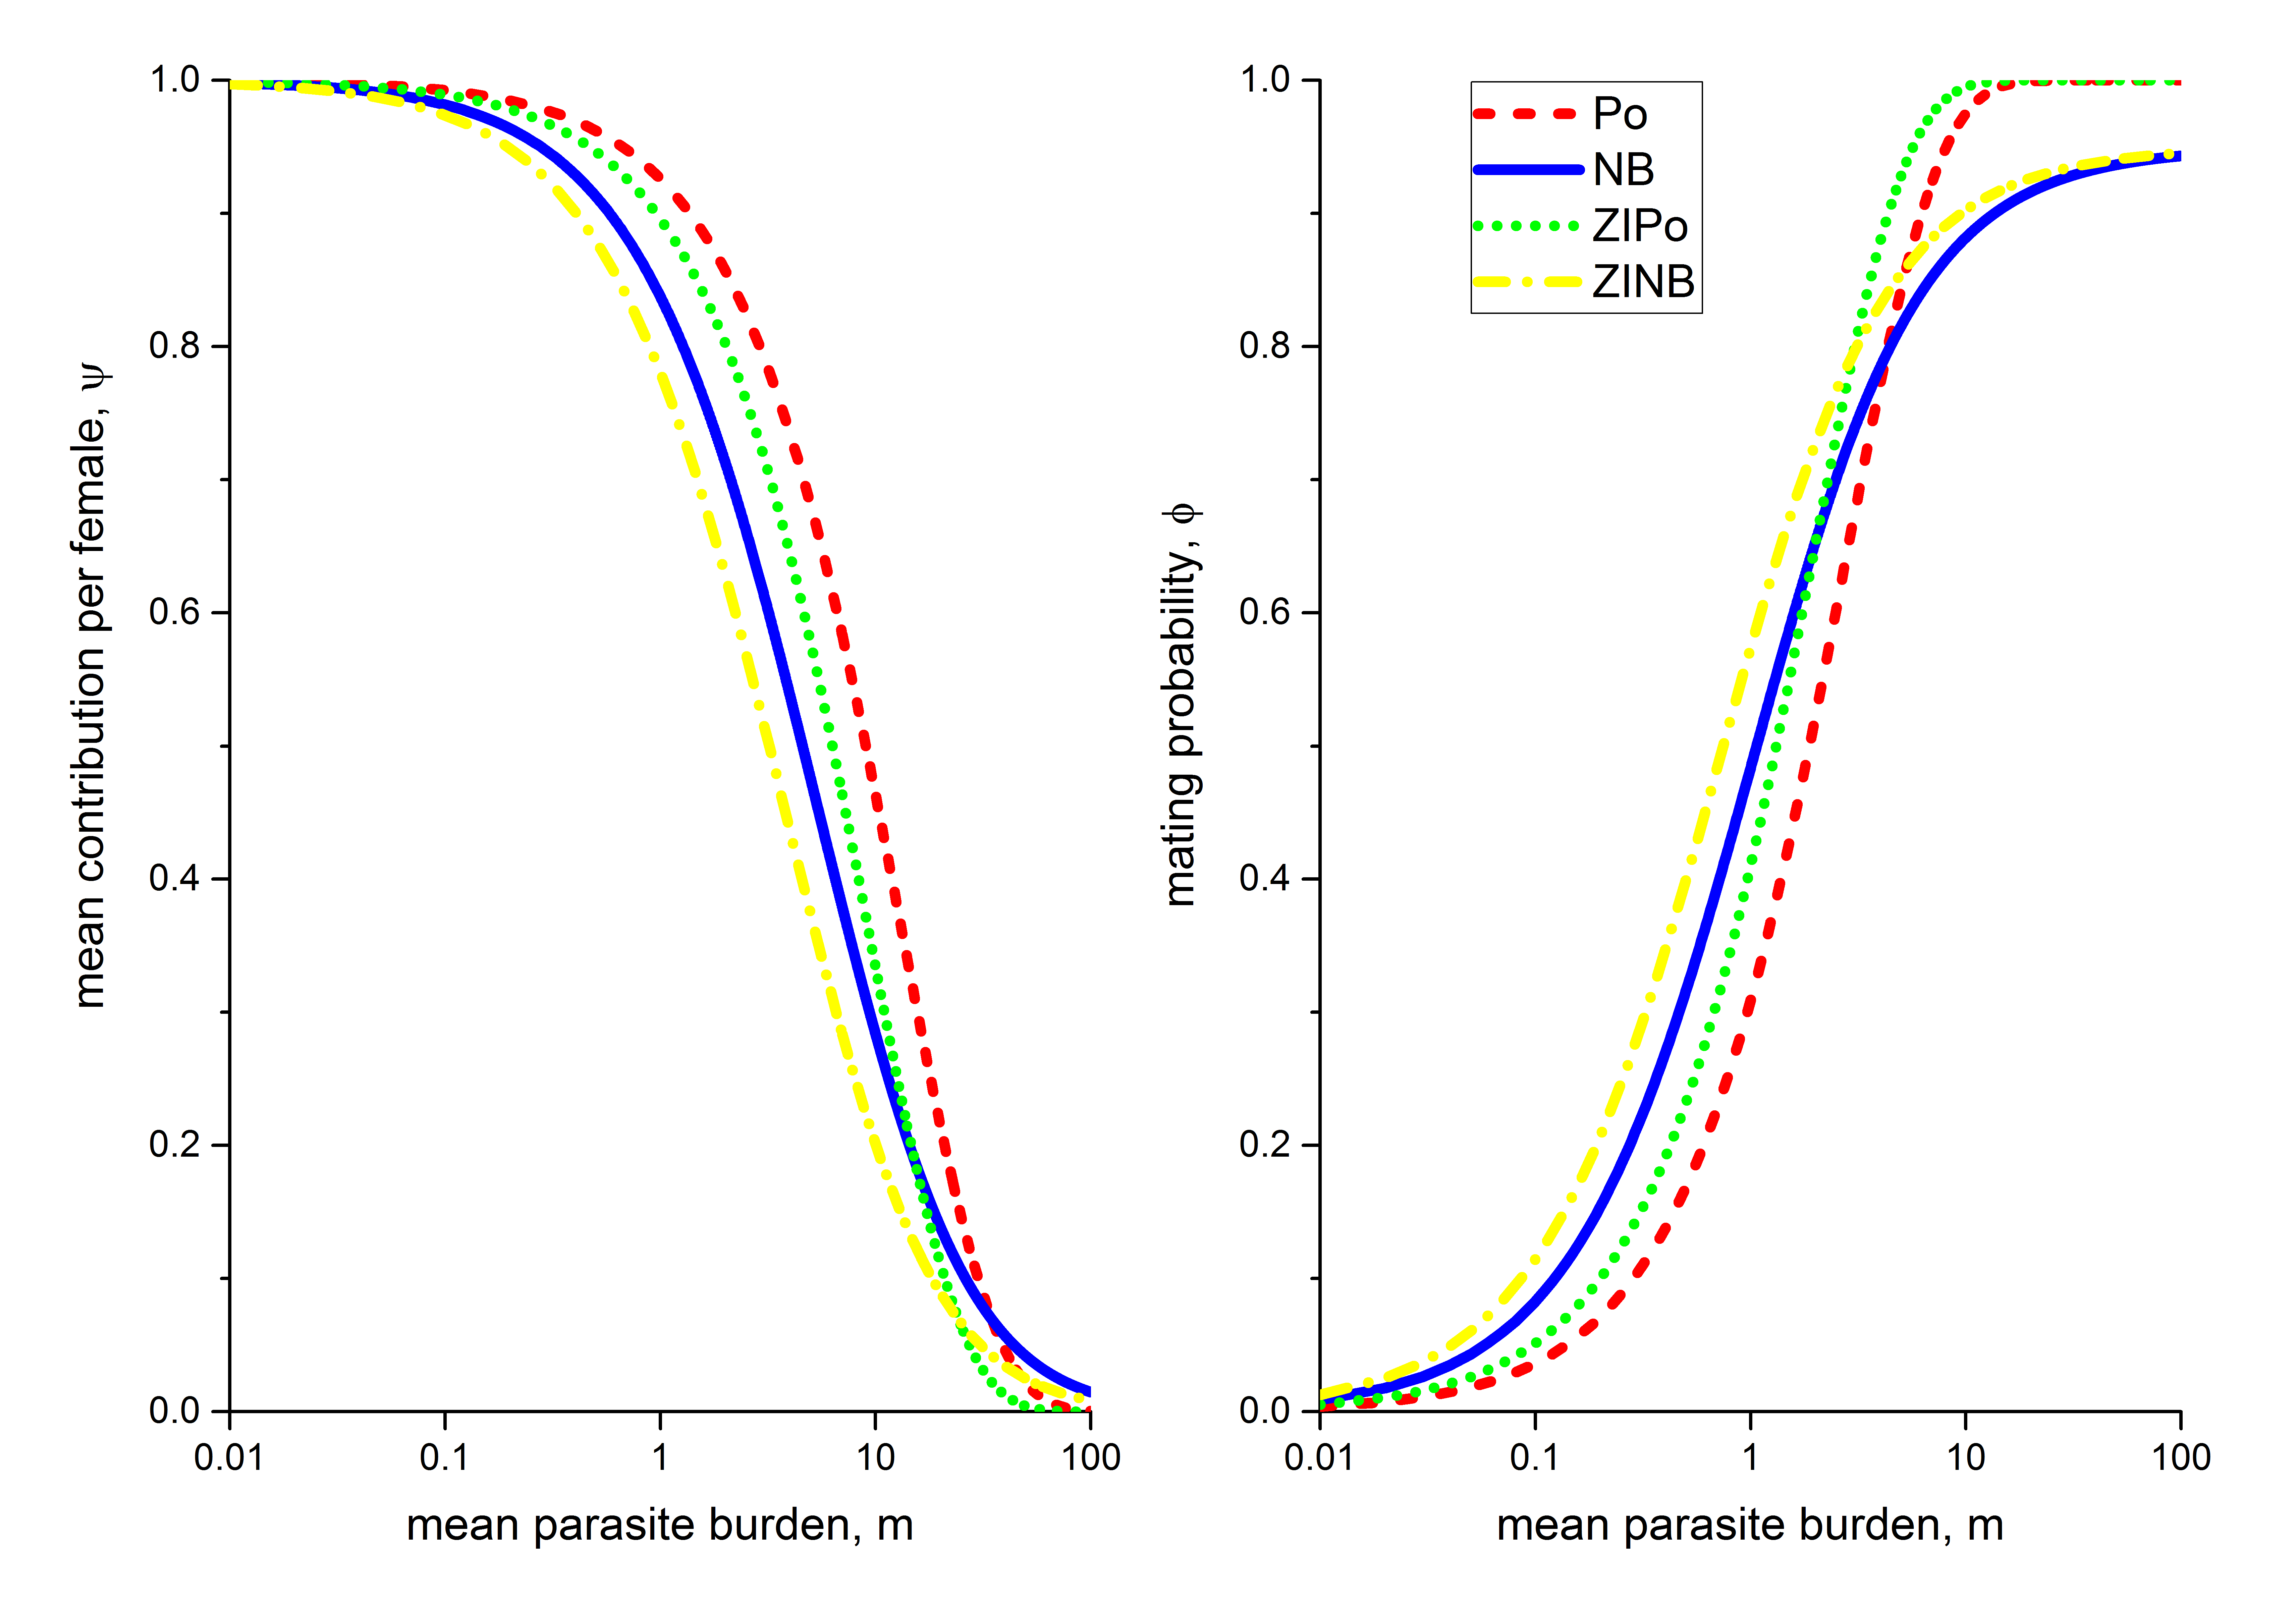
\includegraphics[width=0.99\linewidth]{functionv3}
%	\end{figure}
	
%	\subsection{Otras distribuciones simples}
%	Consideremos primero el caso de la distribución logarítmica, donde su fgp es de la forma 
%	\begin{equation*}
%	\begin{split}
%	G(s)&=\frac{\ln(1-ps)}{\ln(1-p)}\\
%	%G'(s)&=\frac{-1}{\ln(1-p)}\frac{p}{1-ps}
%	\end{split}
%	\end{equation*}
%	Entonces la probabilidad de apareamiento general $\phi$ y  la producción de huevos $\psi$ vienen dadas por las expresiones
%	\begin{equation*}
%	\begin{split}
%	\psi&= \frac{1-p}{1-pz} \\
%	\phi&=1-\frac{1-pz}{1-p\alpha z} 
%	\end{split}
%	\end{equation*}
%	
%	Otro ejemplo es considerar la distribución binomial, con fgp dada por
%	\begin{equation*}
%	\begin{split}
%	G(s)&=\left[1+ p(s-1)\right] ^n \\
%	%G'(s)&=np \left[  1+ p(s-1)\right]^{n-1}
%	\end{split}
%	\end{equation*}
%	Por lo tanto la probabilidad de apareamiento general $\phi$ y  la producción de huevos $\psi$ para este caso estan dadas por 
%	\begin{equation*}
%	\begin{split}
%	\psi&=\left[ 1+ p(z-1)\right]^{n-1} \\ 
%	\phi&=1-\left[\frac{1+ p(\alpha z-1)}{1+ p(z-1)} \right]^{n-1} 
%	\end{split}
%	\end{equation*}
%	A continuación en la Figura \ref{fig:phi} vamos a mostrar un gráfico de la contribución media por hembra $\psi$ y la probabilidad de apareamiento $\phi$ para todas las distribuciones que tratamos.   
%	\begin{figure}[h!]
%		\centering
%		\includegraphics[width=0.49\linewidth]{psinegativa}
%		\includegraphics[width=0.49\linewidth]{mating}
%		\caption{La contribución media por hembra a la izquierda y la probabilidad de apareamiento a la derecha, ambas como función de la carga media de parásitos}
%		\label{fig:phi}
%	\end{figure}

%%%%%%%%%%%%%%%%%%%%%%%%%%%%%%%%%%%%%%%%%%%%%%%%%%%%%%%%%%%%%%%%%%


		
\section{Mating probability  of parasites acquired by skin-penetrating}%Independence in the variables $F$ and $M$}
\label{sec:disindep}

Unlike in section \ref{sec:probapareamiento}, we consider that the transmission of parasites occurs through the skin penetration. This type of transmission occurs in parasites such as Ancylostoma duodenale, Necator americanus, among others \cite{castelletto2014diverso,bryant2018critical}. 

In this type of transmission, the host can acquire a single parasite per infection event. Thus, the host can be infected with only one male or female parasite at a time. Therefore, when analyzing the number of male or female parasites per host, these variables must be independent. Here we will present an analysis of these variables.

	
	%Unlike section \ref{sec:probapareamiento} here, we consider that the transmission of parasites occurs through skin penetration.
	%This type of transmission occurs in parasites such as \textit{Ancylostoma duodenale}, \textit{Necator americanus}, among others.
	
	%In this type of transmission, the host can acquire a single parasite per infection event. Thus, the host can be infected with only one male or female parasite at a time.
	%Therefore, when analyzing the number of male or female parasites per host, these variables must be independent. Here we will present an analysis of these variables.
	
	As in the previous section, let $W$ be the random variable count of the number of parasites in a host and $F$, $M$ are the number of female and male parasites, respectively. 
	In this section we analyze the case in which these variables are independent and therefore verify the following properties
	%In this section, we analyze the case in which these variables are independent, that is, $W$, $F$ and $M$ verifies the following properties
	%
	%Let $W$ be the random variable count of the number of parasites in a host and $F$, $M$ are the number of female and male parasites, respectively.
	%In section \ref{sec:distsexo} we assumed that we know the parasite distribution in host, $W=F+M$, and therefore  the variables F and M are not independent.
	%In section  \ref{sec:distsexo} we assumed that the variables $F$ and $M$ were dependent. 
	%In this section we study the case in which these variables are independent, that is, $W$, $F$ and $M$ verify the following properties
	\begin{equation}\label{independencia}
	\begin{split}
	W&=F+M\\
	G_W(s)&=G_F(s)G_M(s)
	\end{split}
	\end{equation}
	where $G_W$, $G_F$ and $G_M$ are probability generating function of the variables $W$, $F$ and $M$, respectively.
	 
	%The independence of the variables $F$ and $M$ can occur when the parasites are acquired individually, as in case of hookworm parasites that can penetrate the skin of host \cite{paho2022,who2022}.
	%We present all the expressions developed in the section 
	We present an expression for all the variables developed in section
	\ref{sec:probapareamiento}, proofs  are  in the Appendix \ref{formulasind}
	\begin{itemize}
		\item Mean number of fertilized female parasites
		\begin{align}
		%\sum_{i\geq 1}\sum_{j\geq 0} j p_F(j)p_M(i)=
		\alpha m \left[1-p_M(0) \right] 
		\end{align}
		
		\item Mating probability 
		\begin{align}
		%\frac{\sum_{i\geq 1}\sum_{j\geq 0} j p_F(j)p_M(i)}{\sum_{j\geq 0} j p_F(j)}=
		1-p_M(0) 
		\end{align}
		
		\item Mean egg production per host
		\begin{equation}
		\lambda_0G_M(z)G'_F(z)
		\end{equation}
		
		\item Mean fertilized egg production
		\begin{equation}
		\lambda_0 G_M(z) G'_F(z)\left[ 1-\frac{p_M(0)}{G_M(z)}\right]
		\end{equation}
		
		\item Mean effective transmission contribution by female parasite
		\begin{align}
		\psi=\frac{G_M(z)G'_F(z)}{\alpha m}
		\end{align}
		
		\item Mating probability and density-dependence effects
		\begin{equation}
		\phi= 1-\frac{p_M(0)}{G_M(z)}
		\end{equation}
		
		\item Contribution of mean fertilized egg production for mean-based deterministic model  of parasite burden
		 \begin{equation}
		\lambda_0 \alpha m \psi(m) \phi(m)
		\end{equation}
	\end{itemize}
	
	
\subsection{Some examples}
	%Assuming that F and M have the same statistical model, the independence of the variables does not ensure that their sum of these variables
	%corresponds to the same statistical model.

Distributions for the variables $F$ and $M$ are expected to be the same, but with different parameter values if the sex ratio it is not 1:1. However the total parasite burden distribution ($M$), obtained from the conditions (\ref{independencia}), may have a different distribution. 

	
	
	In the examples presented here we show some cases where the variables $W$ , $F$ and $M$ have all the same statistical model.
	We work with some of the most popular distributions	used to model parasites and in all cases and arbitrary sex ratio $\alpha:\beta$, where $\alpha+\beta=1$, it is assumed. 
	
%	Suponiendo que $F$ y $M$ pertenezcan a una misma familia de distribuciones, la independencia de estas variables aleatorias no asegura que la suma pertenezca a esta familia. En los ejemplos que presentaremos aquí se pretende que las variables $W$, $F$ y $M$ pertenezcan a una misma familia de distribuciones.
%	A modo de ejemplo trabajaremos con algunas de las distribuciones más utilizadas. Recordemos que suponemos que las proporciones sexuales de los parásitos \textit{hembra : macho} son $\alpha:\beta$, donde $\alpha+\beta=1$.  
	\subsubsection{Poisson}
	For the case where the distribution of parasites per host is Poisson with mean $\lambda$, that is, $W\sim \mathrm{Po}(\lambda)$. A solution for the independence of variables $F$ and $M$ are the following distributions
	%Para el caso donde la distribución de parásitos en una comunidad de hospedadores sea Poisson con media $\lambda$, es decir, $W\sim \mathrm{Po}(\lambda)$. Una solución de para la independencia de las variables $F$ y $M$ son las siguiente distribuciones       
%	\begin{equation*}
%	F\sim \mathrm{Po}(\alpha \lambda) \qquad M\sim \mathrm{Po}(\beta \lambda)
%	\end{equation*}
%	\begin{align*}
%	G_F(s)G_M(s)&=e^{\alpha\lambda(s-1)}e^{\beta\lambda(s-1)}\\
%	&=e^{(\alpha+\beta)\lambda(s-1)}\\
%	&=e^{\lambda(s-1)}\\
%	&=G_W(s)
%	\end{align*}
	\begin{equation*}
	F\sim \mathrm{Po}(\alpha \lambda) \qquad M\sim \mathrm{Po}(\beta \lambda)
	\end{equation*}
	\begin{align*}
	G_F(s)G_M(s)&=e^{\alpha\lambda(s-1)}e^{\beta\lambda(s-1)}\\
	&=e^{(\alpha+\beta)\lambda(s-1)}\\
	&=e^{\lambda(s-1)}\\
	&=G_{F+M}(s)\\
	&=G_W(s)
	\end{align*}
	Note that the pgf of $F$ and $M$ coincide with what was obtained in section \ref{sec:distsexo}, which shows the independence of these variables in that section.
	We show some of the expressions obtained in the previous section \ref{sec:distsexo} for this case:
	%associated with the distributions by sex	
	%Notemos que las fgp de $F$ y $M$ coincide con la obtenida en la sección \ref{sec:distsexo}, lo cual muestra la independencia de estas variables en esa sección. 
	%Mostramos algunas de las expresiones obtenidas en la sección anterior para el caso de independencia entre las variables asociadas a las distribuciones por sexo %de la carga parasitaria por hospedador 
	\begin{itemize}
	\item Mean effective transmission contribution by female parasite
	\begin{align*}
	\psi=\frac{G_M(z)G'_F(z)}{G'_F(1)}=e^{-m(1-z)}
	\end{align*}
	
	\item Mating probability and density-dependence effects
	\begin{equation*}
	\phi= 1-\frac{p_M(0)}{G_M(z)}=1-e^{- m  z \beta}
	\end{equation*}
	\end{itemize}
	Note that the expression for $\psi$ and $\phi$ are the same as those obtained in the section \ref{sec:ejemplos}.
	%Notemos que la expresión de $\psi$ y $\phi$ son los mismo obtenidos en la sección \ref{sec:ejemplos}.
	
	\subsubsection{Negative binomial}
	
	If $F$ and $M$ are negative binomial distributed with parameters $m_F=\alpha m$, $k_F=\alpha k$, $m_M=\beta m$, $k_M=\beta k$, 
	
	\begin{equation*}
	F\sim \mathrm{NB}(\alpha m,\alpha k) \qquad M\sim \mathrm{NB}(\beta m,\beta k)
	\end{equation*}  
	
	Then the distribution of $W=F+M$ is the negative binomial distribution with parameters $m$ and $k$. In fact,  a solution to problem (\ref{independencia}) is given by
	 
	\begin{align*}
	G_F(s)G_M(s)&=\left[ 1-\frac{\alpha m}{\alpha k}(s-1)\right] ^{-\alpha k} \left[ 1-\frac{\beta m}{\beta k}(s-1)\right] ^{-\beta k}\\
	&=\left[ 1-\frac{m}{k}(s-1)\right] ^{-\alpha k-\beta k}\\
	&=\left[ 1- \frac{m}{k}(s-1) \right] ^{-k}\\
	&=G_{F+M}(s)\\
	&=G_W(s)
	\end{align*}

For this case, the pgf of $F$ and $M$ are not equal to those obtained in section \ref{sec:distsexo}, since it was shown that the variables were not independent. We show some of the expressions obtained in the previous section \ref{sec:distsexo} for case of independence between variables 
	
	\begin{itemize}
		\item Mean effective transmission contribution by female parasite
		\begin{align}
		\psi=\frac{G_M(z)G'_F(z)}{\alpha m}=\left[ 1-\frac{m}{k}(z-1)\right] ^{-(k+1)}
		\end{align}
		
		\item Mating probability and density-dependence effects
		\begin{equation}
		\phi= 1-\frac{p_M(0)}{G_M(z)}=1-\left[ \frac{1+\frac{m}{k}}{1-\frac{m}{k}(z-1)}\right]^{-\beta k} 
		\end{equation}
	\end{itemize}

Note that the expression $\psi$ is the same one obtained in the section \ref{sec:ejemplos}.

	In Figure \ref{fig:funphi} we show the behavior of the mating probability function for the cases in which the female and male parasites are distributed together or independently.

%	\begin{figure}
%		\centering
%		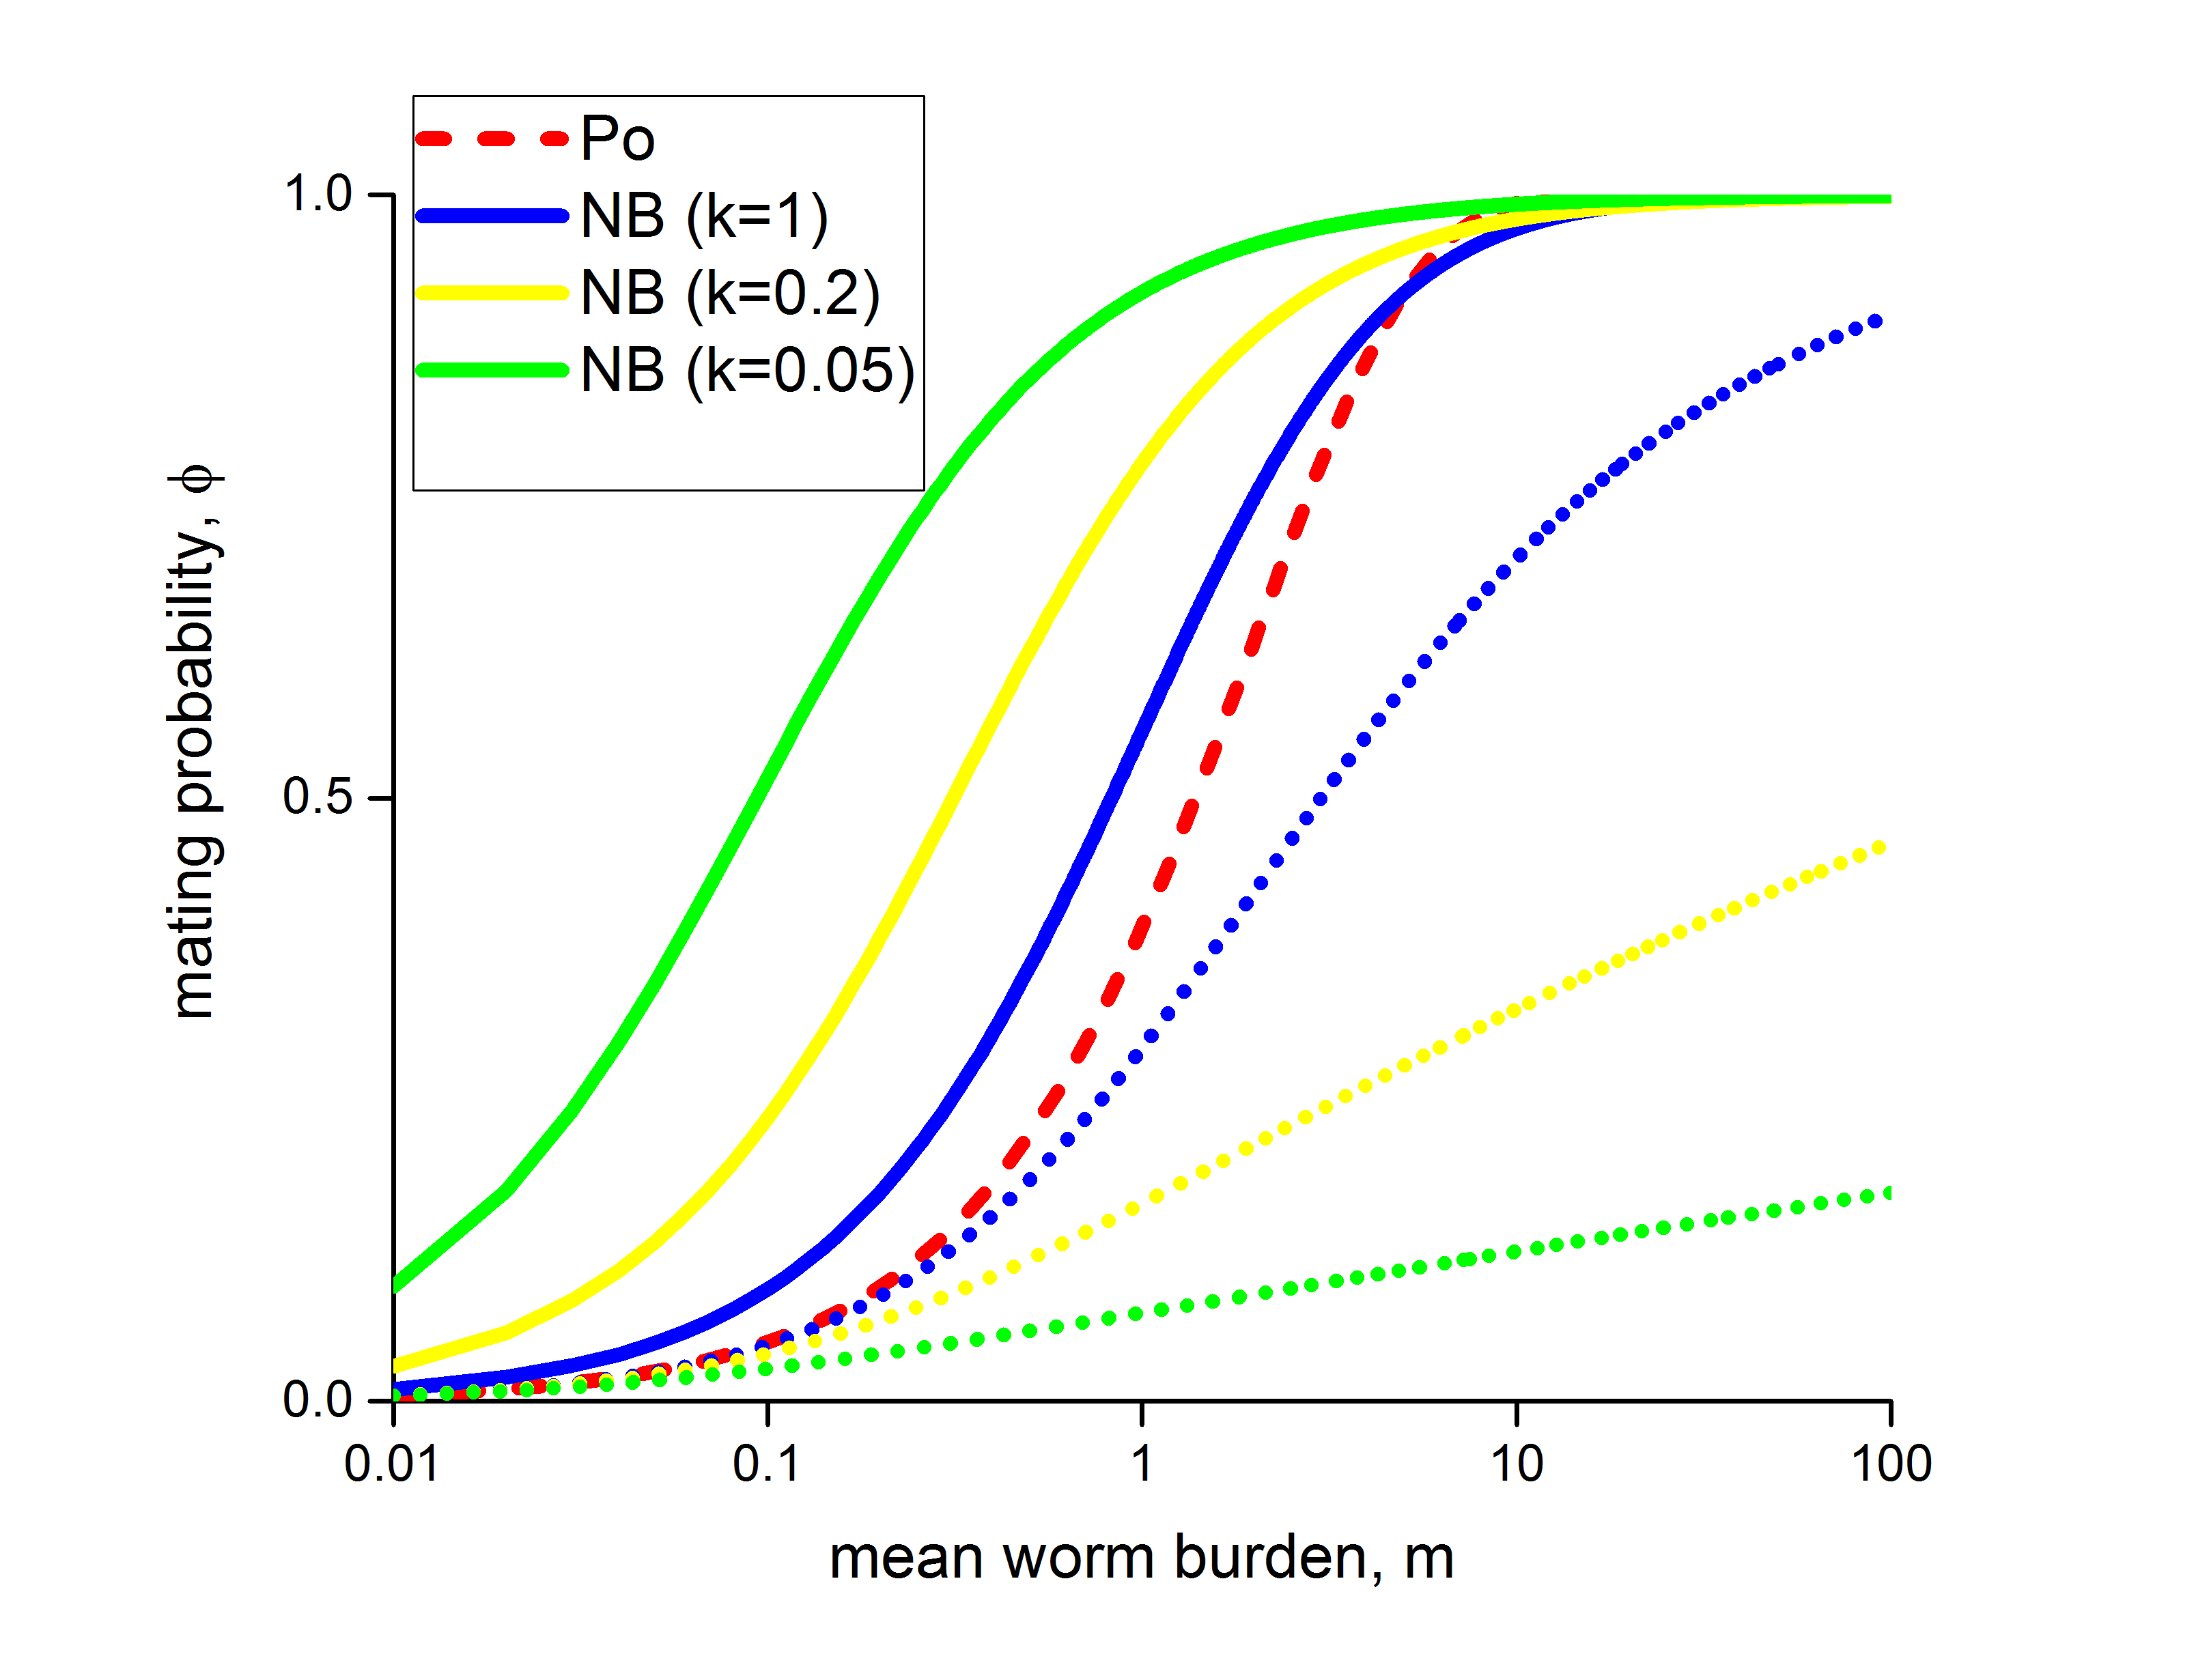
\includegraphics[width=0.99\linewidth]{phiv2}
%		\caption{Mating probability as a function of mean parasite load. The dashed curve (red) corresponds to a Poisson distribution ($k\to \infty$). 
%		%{\color{red}
%		The solid and dotted curves correspond to a negative binomial distribution with joint or independent distribution by sex, respectively, where $k = 1$ (blue), $k =0.2$ (yellow) and $k =0.05$ (green).
%		%}
%		} 
%		\label{fig:funphi}
%	\end{figure}
	
	\section{Computer simulation}
	\subsection{Parasitic infection caused by ingestion of infective eggs}
	For this case we consider that the transmission of parasites is produced by the ingestion of fertilized eggs of these parasites. Here we can consider infection by \textit{Ascaris lumbricoides} and \textit{Trichuris trichiura}.
	
	\begin{itemize}
		\item 
	\end{itemize}
	
	\subsection{Parasitic infection caused by skin-penetrating}
	
	
	\section{Discussion and Conclusions}
	
		
In most cases total macro-parasites distribution is determined by the infection process and therefore the variables $F$ and $M$ (number of female and male parasites within the host) are not independent variables. We presented a general form to obtain the parasite female burden distribution in hosts from the observed total parasite distribution. 	
	
Different reproductive variables of parasites of importance for population dynamics, such as the mean number of fertilized female parasites, mean egg production, mating probability, mean fertilized egg production and mating probability, were obtained. 
	
The  expressions obtained for these reproductive variables in the different examples are generalizations (for the case of density-dependent fertility on reproductive behavior of parasites) of those obtained in\citep{leyton1968stochastic,may1993biased,may1977togetherness}.


%%%%%%%%%%%%%%%%%%%%%%%%%%%%%%%%%%%%

When parasites are acquired individually we expect the random variables $F$ and $M$ to be independent. We also expect that these variables have the same type of distribution. 


But the total host parasite burden $W=F+M$ not necessarily will inherit the same distribution os $F$ amd $M$. There are some obvious cases where it is known that the distribution of the sum of random variables have the same distribution of the the variables like in the case of independent Poisson distributed variables. However for the important case of negative binomial distributed variables this is not generally true. In this work we show that 
%{\color{red} only?} if 
only if
$F\sim \mathrm{NB}(\alpha m,\alpha k)$ and $ M\sim \mathrm{NB}(\beta m,\beta k)$ then the total burden is negative binomial distributed with parameters $m$ and $k$. 


%%%%%%%%%%%%%%%%%%%%%%%%%%%%%%
	
One of the main limitations of this work is that it only considers parasites with a polygamous mating system and we do not consider monogamous and hermaphroditic parasites.

%{\color{red}	
In conclusion, in this work we obtained a general expression for egg production and the mating probability of the parasites. We show how these expressions depend on the sex distribution of the parasites and whether these distributions are considered joint or independent. 
We also show that these expressions vary due to the effects of the density-dependence of the parasites.
%}	
%	Assuming an arbitrary model for distribution of parasites by host, we model the distributions of females and males.
%	We model different reproductive variables of parasites such as mean number of fertilized female parasites, mean egg production, mating probability, mean fertilized egg production and mating probability and density-dependence effects.
%	We show that these reproductive variables depend on independent nature of the $F$ and $M$ variables,  and  density-dependent fecundity of parasites.
%	%We also show that these variables depend on the density-dependent fecundity of each parasite.
%	
%	The reproductive expressions obtained in the examples of this work coincide with those obtained in\citep{leyton1968stochastic,may1993biased,may1977togetherness}.
%	However, in these works, the effects of dense-dependent fertility on reproductive behavior of parasites are not considered.
%	The expressions obtained are a generalization of expressions in \citep{leyton1968stochastic,may1993biased,may1977togetherness}.
%	
%	
%	
%	
%	-What are my most important findings?
%	
%	Asumiendo una distribución arbitraria para la población de parásitos encontramos un expresión para las distribuciones de por sexo (hembra y macho), y partir de estas deducir sus comportamientos reproductivos como el número de hembras fértiles, la producción de huevos y la probabilidad de apareamiento. En todas estas expresiones se consideraron los efectos de denso-dependientes negativos que afectan a la fecundidad del parásito.   
%	
%	-How do my findings compare with what others have found? How consistent are they?
%	
%	
%	Nuestra expresiones obtenidas en este trabajo coinciden con las obtenidas por \cite{may1977togetherness}\cite{may1993biased}\cite{leyton1968stochastic}. Sin embargo en estos trabajos no se considera los efectos que tiene la fecundidad denso-dependiente sobre el comportamiento reproductivo de los parásitos. 
%	
%
%	Nuestras expresiones son una generalización a las obtenidas en los trabajos \cite{may1977togetherness}\cite{may1993biased}\cite{leyton1968stochastic}. 
%
%	si bien nuestra expresiones son genrerales solomente se considre el comportamiento reproductivo de parsitos polygamos , tenemos qeu considrear monogamicos y hermfroditas. 	
	
	
	\section*{Aknowledgements}
	
	This work was partially supported by grant CIUNSA 2018-2467. JPA is a member of the CONICET. GML is a doctoral fellow of CONICET.
	
	\section*{Conflict of Interest}
	
	The authors have declared no conflict of interest.
	
	
	%\section*{References}
	%\newpage
	%\bibliographystyle{plain}
	\bibliographystyle{apa}
	\bibliography{references}	


	\appendix
	\section{Appendix}
	%\section{}
	We will assume that $p$ is the probability mass function of the distribution of parasites per host and $G$ its probability generating function.
	%	En lo que sigue de esta sección supondremos que la 
	%	distribución de parásitos de la población de hospedadores tiene asociada a
	%	$p$ como la función de masa de probabilidad (fmp), mientras que $G$ es la función generadora de probabilidad (fgp). 
	
	\subsection{Mean number of fertilized female parasites}
	\begin{prop}\label{hembrasfecun}
		%Sean $p$ la fmp de la distribución de parásitos y $G$ su fgp, entonces el número medio de parásitos hembra fecundadas por hospedador esta dado por
		The mean number of fertilized female parasites is given by     
		\begin{equation*}
		\alpha  m - \alpha G'(\alpha)
		\end{equation*}
		\begin{proof}
			The presence of at least one male parasite in the host ensures the fertility of all females, so
			%The presence of at least one male parasite in the host ensures that all females will be fertilized, so
			%La presencia de uno o más parásitos macho en el hospedador es suficiente para asegura que todas las hembras serán fecundadas, entonces el número medio de parásitos hembra fecundadas por hospedador esta dado por
			\begin{equation*}
			\begin{split}
			\sum_{n\geq 0}\sum_{j=1}^{n-1}j p_n\binom{n}{j}\alpha^j\beta^{n-j}
			%&=\sum_{n\geq 0}\sum_{j=1}^{n-1}jp(n)\binom{n}{j}\alpha^j\beta^{n-j}\\
			&=\sum_{n\geq 0}p_n\sum_{j=1}^{n-1} j\binom{n}{j}\alpha^j\beta^{n-j}\\
			&=\sum_{n\geq 0}p_n(n\alpha-n\alpha^n)\\
			\end{split}
			\end{equation*}
			where the last line is obtained from the expression of the mean of $\mathrm{B}(n,\alpha)$, $n\alpha=\sum_{j=0}^{n} j\binom{n} {j}\alpha^j\beta^{n-j}$. Therefore
			%donde la ultima linea se obtiene de la expresión de la media de la $\mathrm{B}(n,\alpha)$,  $n\alpha=\sum_{j=0}^{n} j\binom{n}{j}\alpha^j\beta^{n-j}$. Por lo tanto 
			\begin{equation*}
			\begin{split}
			\sum_{n\geq 0}\sum_{j=1}^{n-1}jp_n\binom{n}{j}\alpha^j\beta^{n-j}
			&=\alpha\sum_{n\geq 0}np_n(1-\alpha^{n-1})\\
			&=\alpha \left[ \sum_{n\geq 0}np_n-\sum_{n\geq 0}n\alpha ^{n-1}p_n\right] \\
			&= \alpha  m - \alpha G'(\alpha) 
			\end{split}
			\end{equation*}
		\end{proof}
	\end{prop}
	\subsection{Mean egg production per host}
	\begin{prop}\label{prodhuevos}
		%Sean $p$ la fmp de la distribución de parásitos sobre una población de hospedadores y $G$ su fgp, la producción media de huevos por hospedador esta dada por
		The mean egg production per host is given by
		\begin{equation*}
		\lambda_0\alpha G'(z)
		\end{equation*}
		\begin{proof}
			%Consideramos que todas las hembras presentes en el hospedador pueden producir huevos según su fecundidad per cápita
			We consider that all females present in the host can produce eggs according to their  per-capita fecundity
			\begin{equation*}
			\begin{split}
			\sum_{n\geq 0}\sum_{j=0}^{n}j\lambda(n)p_n\binom{n}{j}\alpha^j\beta^{n-j}
			&=\lambda_0\sum_{n\geq 0}\sum_{j=0}^{n}jz^{n-1}p_n\binom{n}{j}\alpha^j\beta^{n-j}\\
			&=\lambda_0\sum_{n\geq 0}z^{n-1}p_n\sum_{j=0}^{n} j\binom{n}{j}\alpha^j\beta^{n-j}\\
			&=\lambda_0\sum_{n\geq 0}z^{n-1}p_nn\alpha\\
			&=\lambda_0\alpha  \sum_{n\geq 0}nz^{n-1}p_n \\
			&=\lambda_0\alpha G'(z)
			\end{split}
			\end{equation*}
		\end{proof}
	\end{prop}
	
	\subsection{Mean fertilized egg production per host}
	\begin{prop}\label{prodhuevosfecun}
		%Sean $p$ la fmp de la distribución de parásitos sobre una población de hospedadores y $G$ su fgp, la producción media de huevos fecundados por hospedador esta dada por
		The mean fertilized egg production per host is given by
		\begin{equation*}
		\lambda_0\alpha G'(z)\left[1-\frac{G'(\alpha z)}{G'(z)} \right]
		\end{equation*}
		\begin{proof}
			Identical to the previous demonstration but considering only fertilized females
			%Idéntica a la demostración anterior pero considerando solo hembras fecundadas
			\begin{equation*}
			\begin{split}
			\sum_{n\geq 0}\sum_{j=1}^{n-1}j\lambda(n)p_n\binom{n}{j}\alpha^j\beta^{n-j}
			&=\lambda_0\sum_{n\geq 0}\sum_{j=1}^{n-1}jz^{n-1}p_n\binom{n}{j}\alpha^j\beta^{n-j}\\
			&=\lambda_0\sum_{n\geq 0}z^{n-1}p_n\sum_{j=1}^{n-1} j\binom{n}{j}\alpha^j\beta^{n-j}\\
			&=\lambda_0\sum_{n\geq 0}z^{n-1}p_n(n\alpha-n\alpha^n)\\
			%\end{split}
%			\end{equation*}
%			donde la ultima linea se obtiene de la expresión de la media de $\mathrm{B}(n,\alpha)$,  $n\alpha=\sum_{j=0}^{n} j\binom{n}{j}\alpha^j\beta^{n-j}$. Por lo tanto 
%			\begin{equation*}
%			\begin{split}
%			\sum_{n\geq 0}\sum_{j=1}^{n-1}j\lambda(n)p_n\binom{n}{j}\alpha^j\beta^{n-j}
			&=\lambda_0\alpha\sum_{n\geq 0}nz^{n-1}p_n(1-\alpha^{n-1})\\
			&=\lambda_0\alpha \left[ \sum_{n\geq 0}nz^{n-1}p_n-\sum_{n\geq 0}n(\alpha z)^{n-1}p_n\right] \\
			&=\lambda_0\alpha G'(z)\left[1-\frac{G'(\alpha z)}{G'(z)} \right] 
			\end{split}
			\end{equation*}
		\end{proof}
	\end{prop}
	\subsection{Independence in the variables $F$ and $M$}\label{formulasind}
	\begin{itemize}
		\item Mean number of fertilized female parasites
		\begin{align*}
		\sum_{i\geq 1}\sum_{j\geq 0} j p_F(j)p_M(i)
		&=\sum_{i\geq 1}p_M(i)\sum_{j\geq 0} j p_F(j)\\
		&=\left[1-p_M(0) \right] \alpha m
		\end{align*}
		
		\item Mating probability
		\begin{align*}
		\frac{\sum_{i\geq 1}\sum_{j\geq 0} j p_F(j)p_M(i)}{\sum_{j\geq 0} j p_F(j)}
		&=\frac{\left[1-p_M(0) \right] \alpha m }{\alpha m}\\
		&=1-p_M(0) 
		\end{align*}
		
		\item Mean egg production per host
		\begin{align*}
		\sum_{i\geq 0}\sum_{j\geq 1} j \lambda(i+j) p_F(j)p_M(i)
		&=\sum_{i\geq 0}\sum_{j\geq 1} j \lambda_0 z^{i+j-1} p_F(j)p_M(i)\\
		&=\lambda_0\sum_{i\geq 0} z^i p_M(i)\sum_{j\geq 1} j z^{j-1} p_F(j)\\
		&=\lambda_0G_M(z)G'_F(z)
		\end{align*}
		
		\item Mean fertilized egg production per host
		\begin{align*}
		\sum_{i\geq 1}\sum_{j\geq 1} j \lambda(i+j) p_F(j)p_M(i)
		&=\sum_{i\geq 1}\sum_{j\geq 1} j \lambda_0 z^{i+j-1} p_F(j)p_M(i)\\
		&=\lambda_0\sum_{i\geq 1} z^i p_M(i)\sum_{j\geq 1} j z^{j-1} p_F(j)\\
		&=\lambda_0 \left[ G_M(z)-p_M(0)\right]  G'_F(z)\\
		&=\lambda_0 G_M(z) G'_F(z)\left[ 1-\frac{p_M(0)}{G_M(z)}\right]
		\end{align*}
		
		\item Mean effective transmission contribution by female parasite
		\begin{align*}
		\psi=\frac{\sum_{i\geq 0}\sum_{j\geq 1} j \lambda(i+j) p_F(j)p_M(i)}{\sum_{j\geq 1} j p_F(j)}
		&=\frac{G_M(z)G'_F(z)}{\alpha m}
		\end{align*}
		
		\item Mating probability and density-dependence effects
		\begin{equation*}
		\phi= 1-\frac{p_M(0)}{G_M(z)}
		\end{equation*}
	\end{itemize}
	
\newpage

\begin{figure}
	\centering 	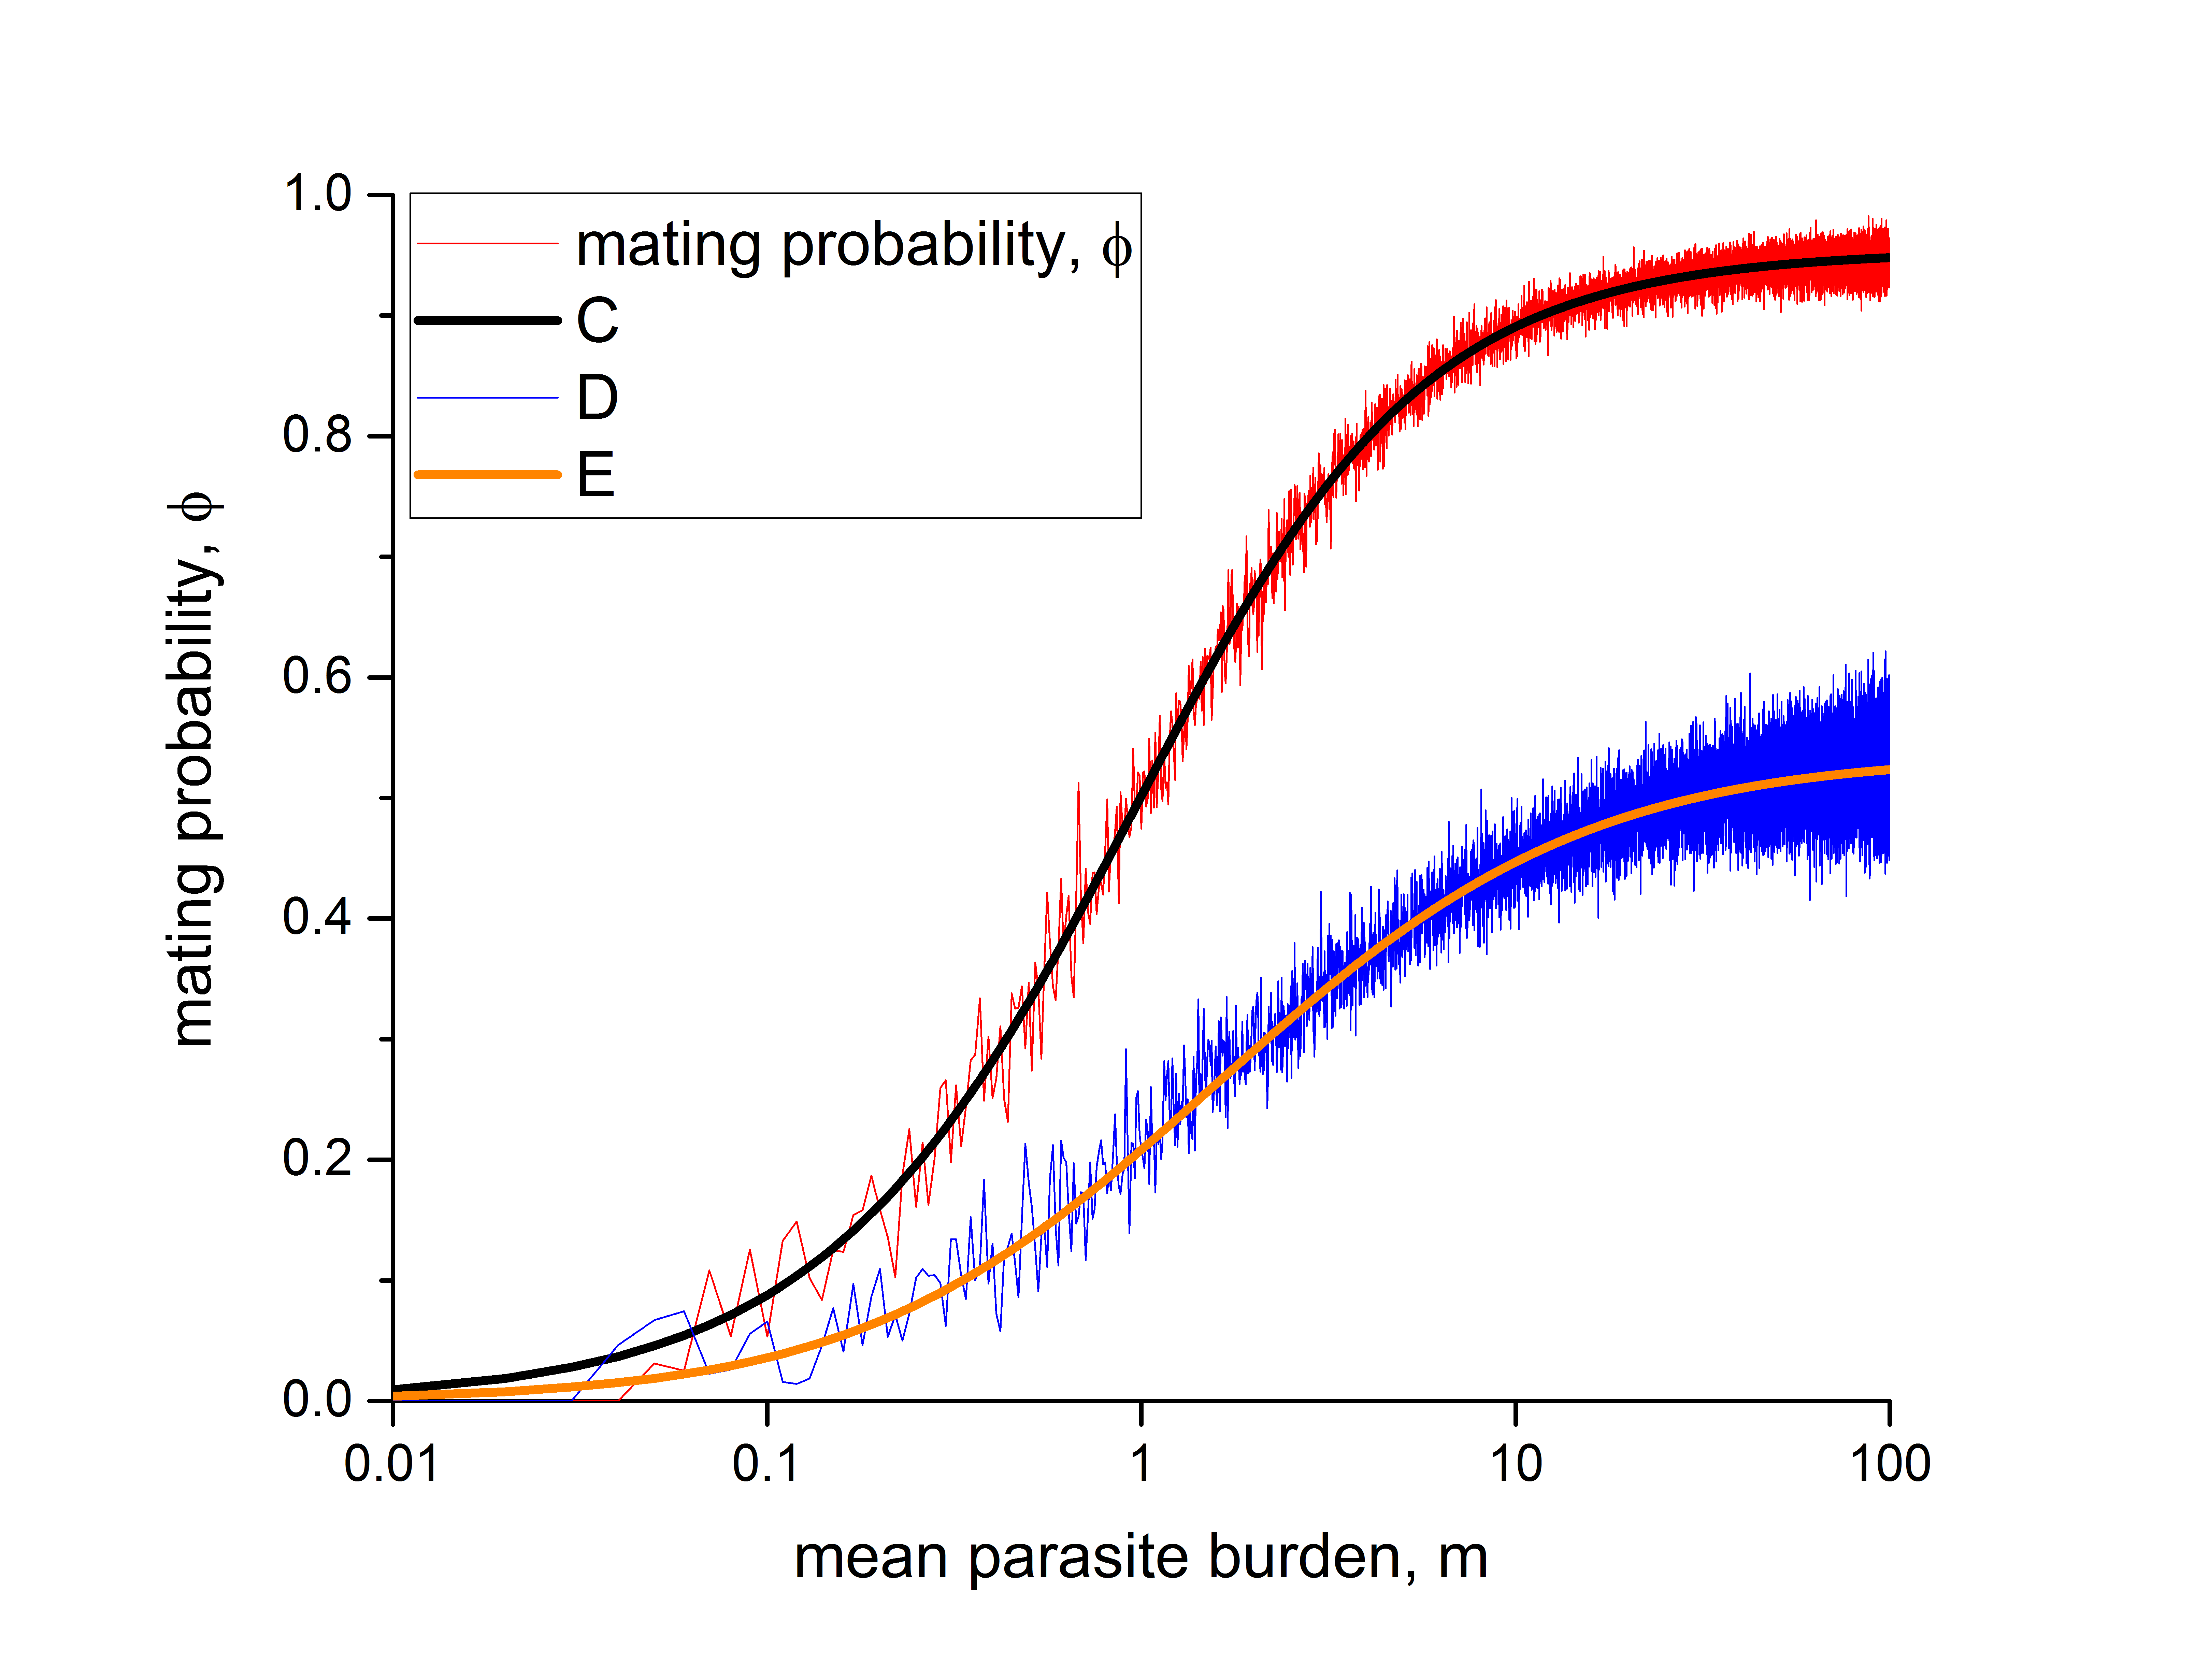
\includegraphics[width=0.9\linewidth]{mating-prob-nb}
	\caption{Mating probability as a function of mean parasite load.
	} 
	%\label{fig:funphi}
\end{figure}


\begin{figure}[h!]
	\centering 	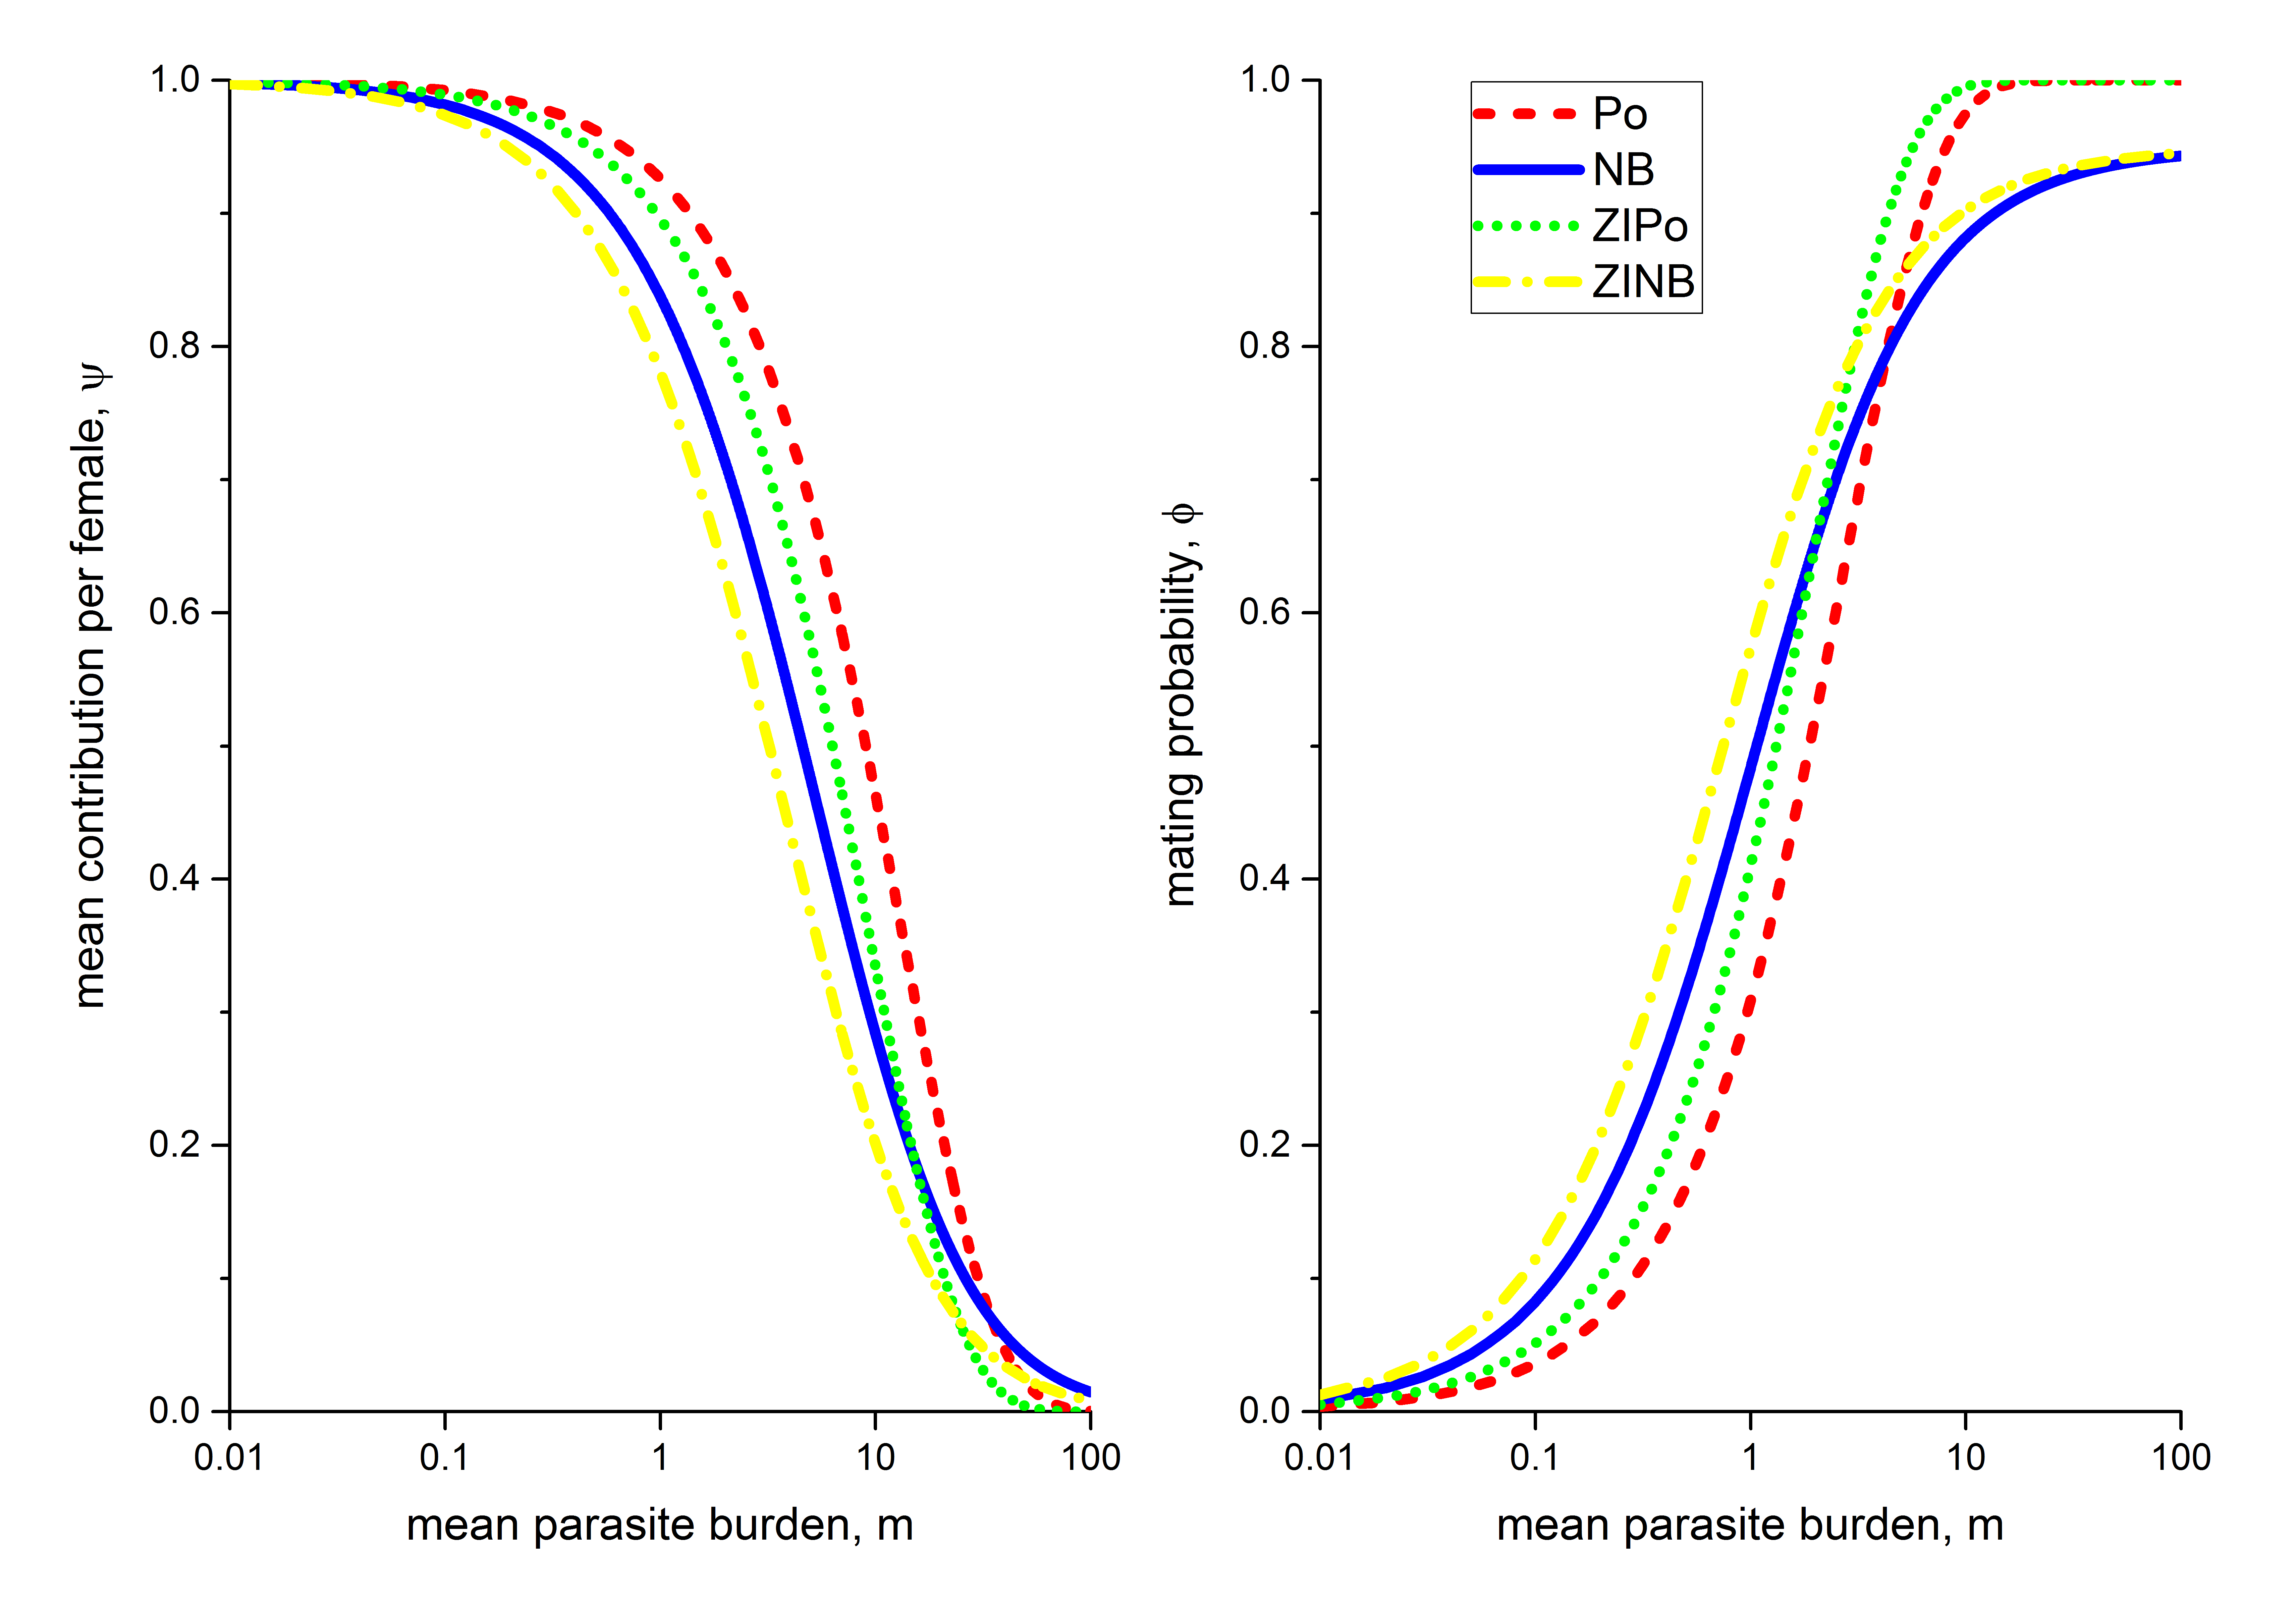
\includegraphics[width=0.99\linewidth]{psiandphi}
	\caption{The mean effective contribution per female parasite, $\psi$ (left) and the mating probability, $\phi$ (right) corresponding to Poisson (dash curve), negative binomial (solid curve), zero-inflated Poisson (dot curve) and zero-inflated negative binomial (dash dot curve) distributions. All as a function of the mean parasite burden $m$.}
	\label{fig:phi}
\end{figure}

\begin{table}[h!]
	\caption{The Effective contribution $\psi$ and the mating probability $\phi$ for zero-inflated Poisson (ZIPo) and zero-inflated negative binomial (ZINB) models.}
	\label{table:function}
	\centering
	\resizebox{\textwidth}{!}{
		%\centering
		\begin{tabular}{c c c}
			\hline  
			\multirow{2}{*}{\minitab[c]{Statistical \\ model}}    & \multirow{2}{*}{effective contribution} & \multirow{2}{*}{mating probability}\\ 
			%\hline
			&  &\\
			\hline
			&  &\\
			ZIPo  & $\psi=\exp\left( \dfrac{m}{1-\pi}(z-1)\right) $ & $\phi=1-\exp\left( -\dfrac{m z \beta}{1-\pi}\right) $	\\ 
			%\hline 
			&  &\\ 
			%\hline 
			ZINB  & $\psi=\left[ 1-\dfrac{m}{k(1-\pi)}(z-1)\right] ^{-(k+1)}$ & $\phi=1- \left[ \dfrac{1-\dfrac{m}{k(1-\pi)}(\alpha z-1)}{1-\dfrac{m}{k(1-\pi)}(z-1)}\right] ^{-(k+1)}$	\\ 
			%\hline 
			&  &\\
		\end{tabular} 
	}
\end{table}

\begin{figure}
	\centering 	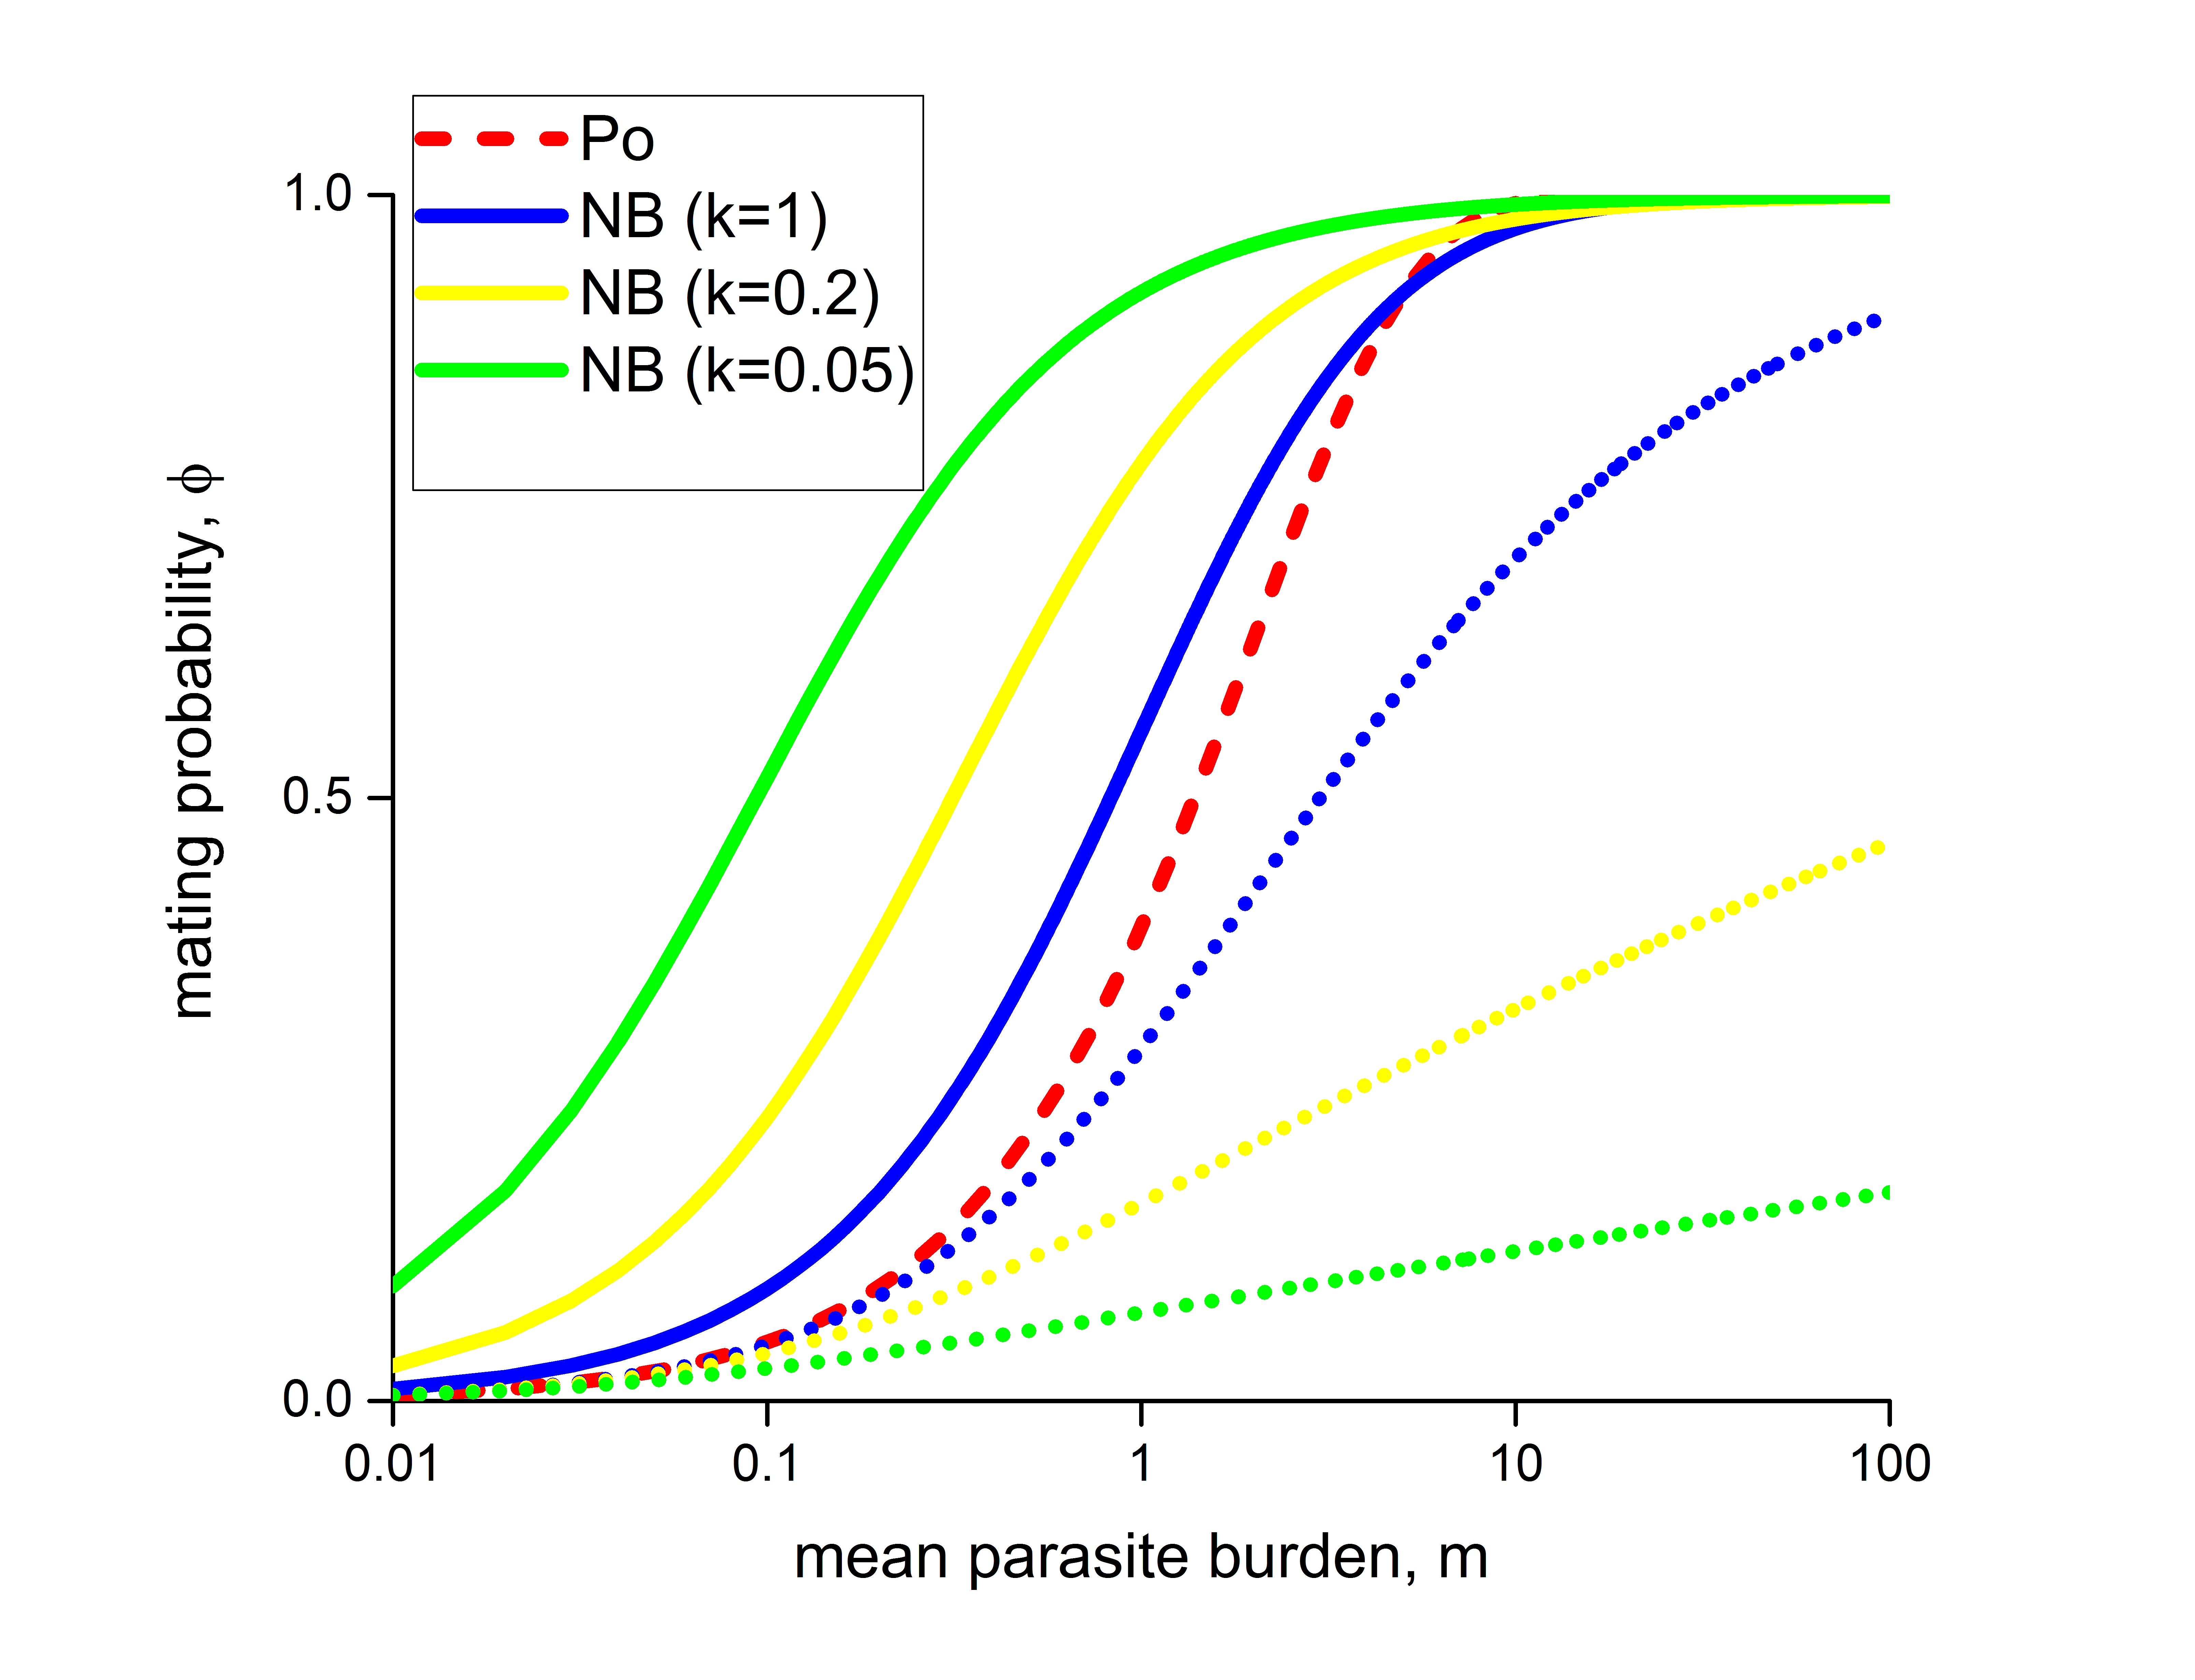
\includegraphics[width=0.9\linewidth]{phi-indep}
	\caption{Mating probability as a function of mean parasite load. The dashed curve (red) corresponds to a Poisson distribution ($k\to \infty$). The solid and dotted curves correspond to a negative binomial distribution with joint or independent distribution by sex, respectively, where $k = 1$ (blue), $k =0.2$ (yellow) and $k =0.05$ (green).
	} 
	\label{fig:funphi}
\end{figure}




\end{document}	
	
	
	
	
	
	
	
	
	
	
	
	
	
	
\section{Distribución de parásitos por sexo}
A partir de obtener la distribución de parásitos en la comunidad de hospedadores también estamos interesados en conocer la distribución de los parásitos según su sexo. 
Suponiendo que las proporciones sexuales para los parásitos hembras y machos son $\varrho$, $1-\varrho$ respectivamente, vamos a estudiar sus distribuciones. 

\subsubsection{Independencia entre la distribución por sexo}	
Suponiendo que un individuo de un comunidad de hospedadores tiene un carga parasitaria según la variable aleatoria
$W$, es natural pensar que esta variable aleatoria se origina como suma de otras dos variables aleatoria independientes $F$ y $M$ que representan la carga parasitaria del hospedador según el sexo del parásito.
Por otro lado de manera experimental es conocido que $W\sim BN(m,k)$ y por las propiedades de las funciones generatrices de probabilidades obtenemos que 
\begin{equation}\label{prop_sexual}
G_W(z)=[1+r(1-z)]^{-k}=G_F(z)G_M(z)
\end{equation}
donde $r=m/k$. Ahora asumiendo que la proporcion sexual de los parásitos es $1:1$ resulta intuitivo pensar las variables aleatorias  
$F$ y $M$ deben ser idénticamente distribuidas resultando 
\begin{equation}
G_F(z)=G_M(z)=G_W(z)^{1/2} 
\end{equation}
es decir que $M,F\sim BN(m/2,k/2)$.

Volviendo al caso mas general donde las proporciones sexuales de los parásitos hembras y machos son $\varrho$ y $1-\varrho$ respectivamente, una solución simple al problema de la ecuación (\ref{prop_sexual}) es
\begin{equation}
F\sim BN(\varrho m,\varrho k) \qquad M\sim BN((1-\varrho) m,(1-\varrho) k)
\end{equation}
dado que    
\begin{align*}
G_F(z)G_M(z)&=\left[ 1+\frac{\varrho m}{\varrho k}(1-z)\right] ^{-\varrho k} \left[ 1+\frac{(1-\varrho) m}{(1-\varrho) k}(1-z)\right] ^{-(1-\varrho) k}\\
&=\left[ 1+r(1-z)\right] ^{-\varrho k-(1-\varrho)k}\\
&=\left[ 1+r(1-z)\right] ^{-k}
\end{align*}

\subsubsection{Producción de huevos}
\begin{align}
p(i)=\sum_{j=0}^i p_F(j)p_M(i-j)
\end{align}

\begin{align}
\sum_{i=0}\varrho i z^{i-1} \left[ \sum_{j=1}^{i-1} p_F(j)p_M(i-j) \right] \\
\sum_{i=0}\varrho i z^{i-1} \left[ p(i)-p_M(0)p_F(i)-p_F(0)p_M(i) \right]\\
\varrho G'(z)-	\varrho p_M(0) G_F'(z) - \varrho p_F(0) G_M'(z)\\
\varrho G'(z)\left[ 1 -	 p_M(0) \frac{G_F'(z)}{G'(z)} -  p_F(0) \frac{G_M'(z)}{G'(z)} \right] 
\end{align}





\subsubsection{No independencia entre la distribución por sexo}	
A diferencia del caso anterior aquí vamos a suponer que para cada individuo 
la carga parasitaria esta dada por la variable aleatoria $W$, la cual origina otras dos variables aleatorias $F$ y $M$ que representan la carga parasitaria del hospedador según el sexo del parásito. Es claro que en este caso estas variables no son independientes, y suponiendo las proporciones sexuales de los parásitos hembras y machos son $\varrho$ y $1-\varrho$ respectivamente 
la esta variables se definen de la siguiente manera
\begin{equation}
F=\sum^W X_i\qquad M=W-F
\end{equation}
donde $X_i\sim Ber(\varrho)$.
Según las propiedades de las funciones generatrices de probabilidades obtenemos que $G_F(z)=G_W(G_{X}(z))$ resulta así que 
\begin{align}
G_F(z)&=G_W(G_{X}(z))\\
&=G_W(1-\varrho+\varrho z)\\
&=[1+r-r(1-\varrho+\varrho z)]^{-k}\\
&=[1+\varrho r-\varrho rz]^{-k}\\
&=[1+(\varrho m/k)-(\varrho m/k)z]^{-k}
\end{align}
obteniendo $F\sim BN(\varrho m,k)$, de manera similar se obtiene que $M\sim BN((1-\varrho) m,k)$

\subsubsection{Producción de huevos}

\begin{equation}
\begin{split}
PH=\sum_{n\geq 0}\sum_{j=1}^{n-1}j\lambda(n)p_n\binom{n}{j}\alpha^j\beta^{n-j}
&=\sum_{n\geq 0}\sum_{j=1}^{n-1}jz^{n-1}p_n\binom{n}{j}\alpha^j\beta^{n-j}\\
&=\sum_{n\geq 0}z^{n-1}p_n\sum_{j=1}^{n-1} j\binom{n}{j}\alpha^j\beta^{n-j}\\
&=\sum_{n\geq 0}z^{n-1}p_n(n\alpha-n\alpha^n)\\
\end{split}
\end{equation}
donde la ultima linea se obtiene de la expresión de la media de la $Bi(n,\alpha)$,  $n\alpha=\sum_{j=0}^{n} j\binom{n}{j}\alpha^j\beta^{n-j}$. Por lo tanto 
\begin{equation}
\begin{split}
PH&=\alpha\sum_{n\geq 0}nz^{n-1}p_n(1-\alpha^{n-1})\\
&=\alpha \left[ \sum_{n\geq 0}nz^{n-1}p_n-\sum_{n\geq 0}n(\alpha z)^{n-1}p_n\right] \\
&=\alpha G'(z)\left[1-\frac{G'(\alpha z)}{G'(z)} \right] 
\end{split}
\end{equation}











\begin{align}
p(i)=\sum_{j=0}^i p_F(j)p_M(i-j)
\end{align}

\begin{align}
\sum_{i=0}\varrho i z^{i-1} \left[ \sum_{j=1}^{i-1} p_F(j)p_M(i-j) \right] \\
\sum_{i=0}\varrho i z^{i-1} \left[ p(i)-p_M(0)p_F(i)-p_F(0)p_M(i) \right]\\
\varrho G'(z)-	\varrho p_M(0) G_F'(z) - \varrho p_F(0) G_M'(z)\\
\varrho G'(z)\left[ 1 -	 p_M(0) \frac{G_F'(z)}{G'(z)} -  p_F(0) \frac{G_M'(z)}{G'(z)} \right] 
\end{align}
